\documentclass[letterpaper, 12pt]{article} %10pt por default
%\usepackage[paper=a4paper,left=24mm,right=24mm,top=20mm,bottom=20mm]{geometry}

\usepackage[utf8]{inputenc}
\usepackage[spanish]{babel}
\usepackage{geometry}
\usepackage{lipsum} %por si hay que hacer pruebas de como se ver\'ia
\usepackage{graphicx}
%\usepackage{rotating}
\usepackage{paracol}
\usepackage{multicol}
\usepackage[numbers]{natbib}
\usepackage{setspace}
\usepackage{xstring}
\usepackage[table,xcdraw]{xcolor}
\usepackage{xargs}
\usepackage{bbding} %para las palomitas
\usepackage{ragged2e}
\usepackage[hidelinks]{hyperref}
\usepackage{wrapfig}
\usepackage{lscape}
\usepackage{rotating}
\usepackage{epstopdf}
\usepackage{amsmath}
\usepackage{amssymb}
%\usepackage{caption}
%\usepackage{subcaption}
\usepackage{subfig}
%\usepackage[ruled,linesnumbered]{algorithm2e}
\usepackage{listings}
%\usepackage[toc, acronym]{glossaries}
\usepackage{verbatim}
\usepackage{float}
\usepackage{enumitem}
\usepackage{mathrsfs}
\usepackage[makeroom]{cancel}
\usepackage[firstpage=true]{background}


\usepackage{tikz}
\usetikzlibrary{positioning,shadows,backgrounds,automata,arrows,arrows.meta}
%\usetikzlibrary{arrows} %arrows meta
%\usepackage{tikz-qtree} % Easy tree drawing tool
%\tikzset{every tree node/.style={align=center,anchor=north}, level distance=2cm} % Configuration for q-trees


\usepackage[breakable]{tcolorbox}



%Para estilo fancy
%\usepackage{fancyhdr}
%\usepackage{lastpage}fenter
%\pagestyle{fancy}
%\fancyhf{}

%\renewcommand{\headrulewidth}{0pt} %Quitar la l\'inea del encabezado de fancy
%\rfoot{\footnotesize{ P\'agina \thepage \hspace{1pt} de \pageref{LastPage} }}





\decimalpoint
%If you use either the babel or polyglossia package you'll have to change the name for the particular language
%you use with babel or polyglossia.
\addto\captionsspanish{% Replace "english" with the language you use
	\renewcommand{\contentsname}{Tabla de contenido}%
	\renewcommand{\listfigurename}{Lista de figuras}
	\renewcommand{\listtablename}{Lista de tablas}
	\renewcommand{\lstlistlistingname}{Lista de programas}
	\renewcommand{\glossaryname}{Glosario}
	% NOMBRES DE FIGURA, TABLA, ETC.
	%\renewcommand{\thefigure}{Fig.(\arabic{figure})}
	\renewcommand{\figurename}{Figura}
	%\renewcommand{\thetable}{Tab.(\arabic{table})}
	\renewcommand{\tablename}{Tabla}
	%\renewcommand{\theequation}{Eq.(\arabic{equation})}
	\renewcommand{\lstlistingname}{Programa}
}
% RENOMBRAR BIBLIOGRAF\'IA
%\renewcommand{\bibname}{\section{Referencias}}
%\renewcommand{\theenumi}{\Alph{enumi}}
\newcommand{\reftab}[1]{Tab.(\ref{#1})}
\newcommand{\reffig}[1]{Fig.(\ref{#1})}
\newcommand{\refeq}[1]{Ec.(\ref{#1})}
\newcommand{\refexp}[1]{Exp.(\ref{#1})}
\newcommand{\refdef}[1]{Def.(\ref{#1})}
\newcommand{\refsec}[1]{Sec.(\ref{#1})}
\newcommand{\refssec}[1]{Subsec.(\ref{#1})}
\newcommand{\refej}[1]{Ej.(\ref{#1})}
\newcommand{\refprog}[1]{Prog.(\ref{#1})}


% SIEMRPE EXISTIR\'A UNA CARPETA IMG
\graphicspath{{./img/}}

% ESPACIO ENTRE COLUMNAS DE MULTICOL
\setlength{\columnsep}{1cm}

% INTERLINEADO
\setstretch{1} %

% SEPARACI\'ON ENTRE P\'ARRAFOS
\setlength{\parskip}{10pt}

% BORRAR SANGR\'IA EN GENERAL
\setlength\parindent{0pt}


% CONFIGURACI\'ON DE HIPERV\'INCULOS
%\hypersetup{
	%    colorlinks=true,
	%    linkcolor=black,
	%    urlcolor=magenta
	%}

% TAMA\~NO DE LA HOJA
\geometry{
	%headsep= 0pt,
	%head=0pt,
	%ignoreall,
	hmargin= {3.5cm, 3.5cm}, %izquierda, derecha
	vmargin= {2.5cm, 2.5cm} %arriba, abajo
}


% PREGUNTA Y RESPUESTA (pregunta dentro de itemizador)
\newcommand{\preg}[1][Pregunta]{
	\item \textbf{#1} \\
}
\newcommand{\resp}[1][Respuesta]{
	\textit{#1} \ \\
}

% ELEMENTO LIBRE DE ITEMIZADOR
\newcommand{\itemlibre}[1]{
	\tab - #1. \\
}

% CONCEPTO DE GLOSARIO: 1->llave, 2->concepto, 3->descripcion
% Requiere libreria glossaries
\newcommand{\itemg}[2]{
	\item \textbf{#1} #2 
	
	\enter
	
}

% ESPACIADORES
\newcommand{\enter}{\vspace{0.5cm}}
\newcommand{\tab}{\hspace{1cm}}

% L\'INEA PARA LLENADO (param: medida de la l\'inea en mm)
\newcommand{\sublinea}[1]{
	\rule{#1mm}{0.1mm}
	<}

% LEYENDAS DE IMAGEN ALTERADAS A CURSIVA
\newcommand{\captionit}[1]{
	\caption{\textit{#1}}
}
\newcommand{\subcaptionit}[1]{
	\subcaption{\textit{#1}}
}

% CUADRO DE REMARCACI\'ON
\newenvironment{remark}[1]{
	\begin{tcolorbox}[
		colback= myNaranja!25,
		colframe= blue254!75,
		title=#1,
		arc= 3mm,
		sharp corners= northwest
		]
		\fontfamily{gag}\selectfont
	}{\end{tcolorbox}}

\newcounter{cteorema}
\newenvironment{theo}[1]{
	\addtocounter{cteorema}{1}
	\begin{tcolorbox}[
		colback=orange!5,
		colframe=blue!50!black,
		title= \textbf{Teorema \thesection.\arabic{cteorema}. #1},
		arc= 3mm,
		sharp corners= north
		]
		\fontfamily{gag}\selectfont
	}{\end{tcolorbox}}

\newcounter{cejemplo}
\newenvironment{ejem}[1]{
	\refstepcounter{cejemplo}
	\begin{tcolorbox}[
		breakable,
		colback=blue!5,
		colframe=blue!75!black,
		title= \textbf{Ejemplo \arabic{cejemplo}. #1},
		arc= 3mm,
		sharp corners= all
		]
		\fontfamily{gag}\selectfont
	}{\end{tcolorbox}}

\newcounter{cdefinicion}
\newenvironment{defon}[1]{
	\addtocounter{cdefinicion}{1}
	\begin{tcolorbox}[
		colback=orange!20,
		colframe=blue254!75,
		title= \textbf{Definici\'on \thesection.\arabic{cdefinicion}. #1},
		arc= 3mm,
		sharp corners= west
		%breakable,
		%enhanced
		]
		\fontfamily{gag}\selectfont
	}{\end{tcolorbox}}



% CONVERSI\'ON DE CONTADORES A GLOBALES
%Para hacer global el contador de figura y no se repita al hacer un paracol
\globalcounter{figure}
\globalcounter{equation}








% COLORES DE PORTADA
\definecolor{myAzul}{HTML}{234ECA}
\definecolor{blue254}{HTML}{02528F}
\definecolor{myVerde}{HTML}{36A736}
\definecolor{myNaranja}{HTML}{FF4312}
\definecolor{guinda}{HTML}{660000}
\definecolor{azul}{HTML}{1A079F}
\definecolor{negro}{HTML}{000000}
\definecolor{blanco}{HTML}{FFFFFF}
\definecolor{dorado}{HTML}{996515}
\definecolor{ududff}{rgb}{0.30196078431372547,0.30196078431372547,1}
\definecolor{template_blue}{HTML}{003473}   % Color of Leiden University logo (Lei-Blauw)
\definecolor{subtitle}{cmyk}{0,0,0,0}       % Color for subtitle (white)
\definecolor{template_text}{HTML}{434655}   % Color for text
\definecolor{template_lightgrey}{HTML}{A8AABC}  % Color of the chapter banner   




% ALINEAR A LA DERECHA LOS N\'UMEROS DE FOOTNOTE
%\footnotemargin{\@makefnmark\hss}




% ESTILO PARA LISTINGS
\definecolor{codegreen}{rgb}{0,0.6,0}
\definecolor{codegray}{rgb}{0.5,0.5,0.5}
\definecolor{codepurple}{rgb}{0.58,0,0.82}
\definecolor{backcolour}{rgb}{0.95,0.95,0.92}

\lstdefinestyle{mystyle}{
	backgroundcolor=\color{backcolour},   
	commentstyle=\color{codegreen},
	keywordstyle=\color{magenta},
	numberstyle=\tiny\color{codegray},
	stringstyle=\color{codepurple},
	basicstyle=\ttfamily\footnotesize,
	breakatwhitespace=false,         
	breaklines=true,                 
	captionpos=b,                    
	keepspaces=true,                 
	numbers=left,                    
	numbersep=5pt,                  
	showspaces=false,                
	showstringspaces=false,
	showtabs=false,                  
	tabsize=1
}

\lstset{style=mystyle}




\makeatletter
\newcommand\binomialCoefficient[2]{%
	% Store values 
	\c@pgf@counta=#1% n
	\c@pgf@countb=#2% k
	%
	% Take advantage of symmetry if k > n - k
	\c@pgf@countc=\c@pgf@counta%
	\advance\c@pgf@countc by-\c@pgf@countb%
	\ifnum\c@pgf@countb>\c@pgf@countc%
	\c@pgf@countb=\c@pgf@countc%
	\fi%
	%
	% Recursively compute the coefficients
	\c@pgf@countc=1% will hold the result
	\c@pgf@countd=0% counter
	\pgfmathloop% c -> c*(n-i)/(i+1) for i=0,...,k-1
	\ifnum\c@pgf@countd<\c@pgf@countb%
	\multiply\c@pgf@countc by\c@pgf@counta%
	\advance\c@pgf@counta by-1%
	\advance\c@pgf@countd by1%
	\divide\c@pgf@countc by\c@pgf@countd%
	\repeatpgfmathloop%
	\the\c@pgf@countc%
}
\makeatother













\newcommand{\pnormal}[3]{
	\backgroundsetup{
		scale=1,
		opacity= 0.05,
		angle= 0,
		contents= {
			
\includegraphics[width=0.75\paperwidth, height=0.9\paperheight]{../portada.tex/logo_ipn_negro.png}
		}
	}
	\BgThispage
	\begin{center}
   		\begin{figure}[!tbp]
   			\centering
   			\subfloat{
\includegraphics[scale=0.2]{../portada.tex/logo_cic.png}}
   			\hfill
   			\subfloat{
\includegraphics[scale=0.2]{../portada.tex/logo_cic.png}}
   		\end{figure}
        
        {\LARGE \textcolor{guinda}{\textbf{I}NSTITUTO \textbf{P}OLIT\'ECNICO \textbf{N}ACONAL} }
        \\ \vspace{1cm}
        {\LARGE \textit{ \textcolor{azul}{Centro de Investigaci\'on en Computaci\'on} } }
		\\
        {\Large \textit{ \textcolor{azul}{(\textbf{CIC})} } }
        \\ \vspace{2.5cm}
        {\Large \textsc{\underline{#1}}} %%%%%%%%%%Materia%%%%%%%%%%
        \\ \vspace{2.5cm}
        {\LARGE \textbf{ \textcolor{guinda}{#2} } } %%%%%%%%%%Título%%%%%%%%%%
        \\ \vspace{2.5cm}
        {\Large \textsc{ #3 } } %%%%%%%%%%Profesor%%%%%%%%%%
        \\ \vspace{2cm}
        {\Large \textsc{ Manuel Emilio Ben\'itez Morales } }
        %\ \\
        %A230720
        \\ \vspace{2cm}
        {\large \textsc{  \textsl{ Ciudad de M\'exico, \today } } }
    \end{center}
}


\begin{document}
	\pagenumbering{gobble}
	\pnormal
	{Sistemas operativos}
	{Proyecto final. \\ Análisis de código e instalación del sistema operativo OpuntiaOS en una arquitectura ARM o x86.}
	{Dr. José Luis Oropeza Rodríquez}
	\tableofcontents
	
	\pagenumbering{arabic}
	
	\newpage \section{Antecedentes}

OpuntiaOS es un sistema operativo gratuito, de código abierto, disponible
en su 
\href{https://github.com/opuntiaOS-Project/opuntiaOS}{\textcolor{blue}{repositorio}}
de \texttt{GitHub}.

% x86/x86-64, ARMv7 and Arm64 kernel with pre-emptive multi-threading



De acuerdo con su descripción en \cite{osdev} (\texttt{ctrl+F} -> ``opuntiaOS''):
\begin{center}
	\begin{minipage}{10cm}
		\itshape
		``opuntiaOS - un sistema opetativo que soporta x86 y ARMv7. Proporciona un kernel con excelentes características como SMP and Ext2, bibliotecas de tiempo de ejecución personalizadas para C/C++/ObjC y bibliotecas para UI.''
	\end{minipage}
\end{center} 



De la misma manera, se menciona que el desarrollo del \textit{kernel} está activo
y observando el repositorio, la última actualización de código fue el 06 de Abril del 2023.



Este sistema contiene un \textit{Prickly Pear Kernel}, que en términos estrictos de sistemas operativos no tiene un significado en específico, sin embargo, en el repositorio del autor (\texttt{docs/kernel.md}) se menciona que:
\begin{center}
	\begin{minipage}{10cm}
		\itshape
		``Prickly Pear Kernel de opuntiaOS es un kernel similar a Unix, que soporta arquitecturas x86/x86-64, arm32 y arm64.''
	\end{minipage}
\end{center}



Los principales directorios, relacionados con la teoría del curso, son:
\begin{itemize} \setlength\itemsep{0pt}
	%\item \texttt{algo}: Algoritmos y estructuras usadas por el \textit{kernel}.
	\item \texttt{drivers}: Controladores de las plataformas soportadas.
	\item \texttt{fs}: Implementación del VFS y FS soportados.
	%\item \texttt{io}: Elementos de comunicación.
	%\item \texttt{libkern}: Librería de soporte para el \textit{kernel}.
	\item \texttt{mem}: Manejadores de memoria física y virtual.
	\item \texttt{platform}: Código para la arquitectura \texttt{ARM}.
	\item \texttt{syscalls}: Implementación de \texttt{syscalls}.
	%\item \texttt{tasking}: Mecanismos de control de tareas.
	\item \texttt{time}: Manejador de tiempo.
\end{itemize}



\newpage
\subsection{Ninja \label{ssec:ninja}}
	\texttt{Ninja} es un sistema de construcción pequeño centrado en la velocidad que, a diferencia de otros sistemas de compilación, está diseñado para que sus archivos de entrada sean generados por un sistema de compilación de nivel superior y está diseñado para ejecutar compilaciones lo más rápido posible \cite{ninja}.
	
	Mientras que otros sistemas de compilación, como \texttt{make}, son lenguajes de alto nivel, \texttt{Ninja} pretende ser un ensamblador \cite{ninja}. 
	
	Este enfoque de bajo nivel lo hace perfecto para integrarlo en sistemas de construcción con más funciones. \texttt{Ninja} se usa para construir Google Chrome, partes de Android, LLVM y se puede usar en muchos otros proyectos gracias al \textit{backend} \texttt{Ninja} de \texttt{CMake} \cite{ninja}.
	
	La última versión de \texttt{Ninja} es la 1.11.1, disponible en su repositorio de Github, sin embargo, es accesible desde los repositorios de Ubuntu por medio de \texttt{sudo apt install ninja-build} pero su versión más reciente es la 1.10.1-1.
	
\subsection{GN \label{ssec:gn}}
	GN es un sistema de meta-contrucción que genera archivos de construcción para \texttt{Ninja},  se utiliza actualmente como sistema de construcción para Chromium, Fuchsia y proyectos relacionados
	\cite{gn}.
	
	Está diseñado para proyectos multiplataforma y admite múltiples directorios de salida paralelos, cada uno con su propia configuración. Esto permite que un desarrollador mantenga compilaciones de depuración, liberación o plataformas diferentes en paralelo sin reconstrucciones forzadas al cambiar de directorio \cite{gn}.
	
	También comprueba las dependencias, entradas y salidas, permitiendo garantizar que la compilación evolucione según lo deseado \cite{gn}.
	
\newpage
\subsection{LLVM \label{ssec:llvm}}
	Es una colección de tecnologías modulares y reutilizables de compiladores y herramientas que comenzó como un proyecto de investigación en la Universidad de Illinois, con el objetivo de proporcionar una estrategia de compilación moderna basada en 
	SSA\footnote{
		\textit{Static Single Assignment}  es un medio para estructurar la representación intermedia, de modo que cada variable se asigne un valor solo una vez y cada variable se define antes de su uso, su utilidad es simplificar y emjorar los resultados de los algoritmos de optimización del compilador \cite{ssa_gfg}.
	}
	
	capaz de apoyar la compilación estática y dinámica de lenguajes de programación arbitrarios \cite{llvm}. 
	
	\texttt{LLVM} se ha convertido en un proyecto general que consiste en una serie de subproyectos, muchos de los cuales están siendo utilizados en producción de otros más comerciales y de código abierto \cite{llvm}.
	
	
	
	Además, es ampliamente utilizado en la investigación académica. El código en el proyecto \texttt{LLVM} tiene licencia \texttt{Apache 2.0} con excepciones \texttt{LLVM} \cite{llvm}.
	
\subsection{QEMU}
	Es un emulador de máquina y espacio de usuario y virtualizador genérico de código abierto, capaz de emular máquinas sin necesidad de soporte de virtualización de hardware \cite{qemu_repo}. 
	
	
	
	Utiliza 
	traducción dinámica\footnote{
		La traducción dinámica es una técnica que permite ejecutar código binario de una arquitectura de CPU en una arquitectura diferente, traduciendo las instrucciones del código binario original a las instrucciones de la arquitectura del equipo anfitrión en tiempo real \cite{qemu_kvm}.
	}
	, logrando un buen rendimiento y puede integrarse con los aceleradores de \textit{hardware} \texttt{Xen} y \texttt{KVM} para proporcionar \textit{hardware} emulado y al mismo tiempo permitir que el acelerador administre la CPU \cite{qemu_repo}.
	
	
	
	``Cuando \texttt{QEMU} emula CPU directamente, es capaz de ejecutar sistemas operativos creados para una máquina (por ejemplo, una placa ARMv7) en una máquina diferente (por ejemplo, una placa de PC x86\_64)'' \cite{qemu_repo}.
	


	
	
	
	

	\newpage \section{Objetivos}



\subsection{General}
Analizar y comprender la manera en que el sistema operativo OpuntiaOS arranca en 
una arquitectura ARM, poniendo especial énfasis en el \textit{bootloader}.



\subsection{Específicos}
\begin{itemize} \setlength\itemsep{0pt}
	\item Emular \texttt{OpuntiaOS} en la herramienta \texttt{QEMU}.
	\item Comprender la manera en que se implementa el \textit{bootloader} 
	para poder dar control a \texttt{OpuntiaOS}.
	\item Realizar una comparación de la forma  de arranque en x86 contra ARM.
	\item Arrancar \texttt{OpuntiaOS} en una tarjeta con arquitectura \texttt{ARM}.
	\item Describir y relacionar las características anteriores, en \texttt{OpuntiaOS}, con aquellas descritas
	durante el curso.
\end{itemize}



	\newpage \section{Requerimientos previos \label{sec:reqPrevios}}
Los requerimientos previos se consideran para la compilación del sistema en
\texttt{Ubuntu 22.04.3 LTS}, entonces se coloca en esta sección las instrucciones 
para dicha distribución.

\subsection{Instalación de herramientas}
	Debido a que \texttt{GN} utiliza \texttt{Ninja} y, en general, para la 
	compilación del \textit{kernel} se utilizan las utilidades de GNU y otras
	librerías de desarrollo, es conveniente instalar todas estas herramientas antes de continuar a los requerimientos posteriores.
	
	
	
	En el repositorio del autor se menciona, en el archivo \texttt{docs/build.md}, sección \textit{Tools for Linux (Ubuntu)}, que las
	herramientas se instalan por medio de:
	\begin{center}
		\ttfamily
		apt install build-essential curl libmpfr-dev libmpc-dev libgmp-dev e2fsprogs qemu-system-i386 qemu-utils nasm fuseext2 ninja,
	\end{center}

	
	
	sin embargo, funciona mejor utilizar lo siguiente:
	\begin{center}
		\ttfamily
		sudo apt install build-essential curl libmpfr-dev libmpc-dev libgmp-dev e2fsprogs nasm fuseext2 ninja-build.
	\end{center}

	
	
	Por otro lado, se require también la instalación de \texttt{Python}, la distribución donde se compiló \texttt{OpuntiaOS}, así como otras recientes, ya lo
	traen instalado por defecto, sin embargo, puede instalarse como:
	\begin{center}
		\ttfamily
		sudo apt install python3.
	\end{center}


\subsection{Instalación de QEMU \label{ssec:installQuemu}}
	De acuerdo con el repositorio del autor (\texttt{docs/getting\_qemu.md}), debe 
	instalarse el emulador \texttt{QEMU} por medio de la siguiente línea:
	\begin{center}
		\ttfamily
		apt install qemu-utils qemu-system-i386 qemu-system-x86\_64 qemu-system-arm,
	\end{center}

	
	
	sin embargo, en la versión donde se llevó a acabo la compilación se debe 
	instalar como sigue:
	\begin{center}
		\ttfamily
		sudo apt install qemu-utils qemu-system-x86 qemu-system-arm.
	\end{center}

	
	De esta manera se tendrán disponibles las siguientes instrucciones 
	del sistema:
	\begin{itemize} \setlength\itemsep{0pt}
		\item \textbf{\texttt{qemu-system-x86\_64}},
		\item \textbf{\texttt{qemu-system-i386}},
		\item \texttt{qemu-system-aarch64},
		\item \textbf{\texttt{qemu-system-arm}}.
	\end{itemize}



\subsection{Instalación de GN \label{ssec:installGn}}
	\texttt{OpuntiaOS} utiliza GN como sistema de construcción, para instalarlo debe obtenerse su código fuente, el enlace se menciona tanto en el repositorio de
	\texttt{OpuntiaOS} (\texttt{docs/getting\_gn.md}) como en \cite{gn}.
	
	
	
	En el repositorio de \texttt{OpuntiaOS} se hace uso del comando \texttt{python}, sin embargo, resulta mejor opción utilizar \texttt{python3}, o bien, hacer un enlace simbólico que apunte al binario de \texttt{python3}.
	
	
	
	Después de validar que \texttt{Python} está disponible, puede proceder la 
	instalación tal como menciona el archivo \texttt{docs/getting\_gn.md}.
	\begin{figure}[ht]
		\centering
		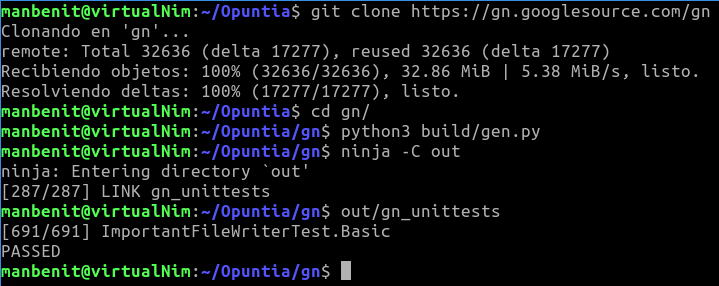
\includegraphics[scale=0.4]{installGn.png}
		\caption{
			Proceso de instalación de \texttt{GN}.
			\label{fig:installGn}
		}
	\end{figure}




\newpage
\subsection{Instalación de LLVM}
	Para instalar \texttt{LLVM} se requiere un archivo ejecutable que puede 
	conseguirse por medio de \texttt{wget}, esto se menciona en el repositorio de \texttt{OpuntiaOS} (\texttt{docs/build.md}).
	\begin{figure}[ht]
		\centering
		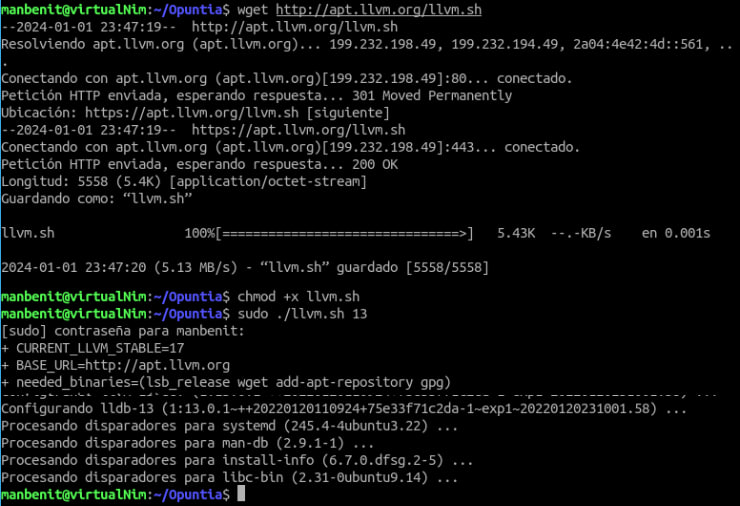
\includegraphics[scale=0.51]{installLlvm.jpg}
		\caption{
			Proceso de instalación de \texttt{LLVM}.
			\label{fig:installLlvm}
		}
	\end{figure}


\subsection{Instalación de dependencias de Python}
	En el archivo \texttt{docs/build.md} también se menciona la instalación de
	las dependencias:
	\begin{itemize} \setlength\itemsep{0pt}
		\item \texttt{construct}, versión 2.10.67,
		\item \texttt{gitpython}, versión 3.1.27,
		\item \texttt{pyelftools}, versión 0.28,
	\end{itemize}
	
	
	
	que se especifican en el archivo 
	\texttt{utils/python\_requirements.txt},
	y de la misma manera que en la \autoref{ssec:installGn}, se recomienda usar la versión reciente, en este caso, del gestor de paquetes (\texttt{pip3}), en lugar del \texttt{pip} mencionado en el repositorio.
	
	
\newpage
\subsection{Instalación del \textit{toolchain} para x86}
	Se deben asignar permisos de ejecución al \textit{script} de instalación por medio de 
	\begin{center}
		\ttfamily
		chmod 775 toolchains/scripts/i686-elf-tools.sh,
	\end{center}

	este archivo se referencia en \texttt{docs/build.md}, sección \textit{GNU Toolchain for Linux (Ubuntu)}, del repositorio de \texttt{OpuntiaOS}.
	
	
	
	El \textit{script} se encarga de:
	\begin{itemize} \setlength\itemsep{0pt}
		\item Guarda la ruta de construccion en HOME
		\item guarda la ruta de construcción en la variable de entorno del sistema.
		\item Instalar paquetes útiles para la compilación futura del sistema, varias de ellas es probable que ya vengan pre-instaladas por defecto.
		
	\end{itemize}

	En la función \texttt{installPackages} se intenta instalar \texttt{Python}, pero debe cambiarse el nombre del paquete a \texttt{python3}, porque en distribuciones recientes como en la que se compiló el sistema se utiliza la forma reciente (\texttt{python3}).
	\begin{figure}[ht]
		\centering
		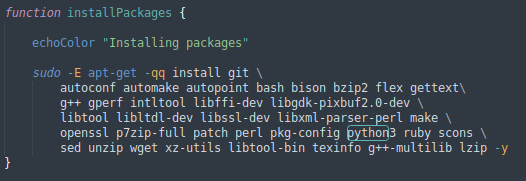
\includegraphics[scale=0.55]{modificarPython.png}
		\caption{
			Modificación de \texttt{python} a \texttt{python3} en la función \texttt{installPackages} de \texttt{i686-elf-tools.sh}.
			\label{fig:modificarPython}
		}
	\end{figure}

	\newpage
	
	Finalmente debe ejecutarse como indica el repositorio:
	\begin{center}
		\ttfamily
		./toolchains/scripts/i686-elf-tools.sh,
	\end{center}
	cuya ejecución se muestra en la \autoref{fig:toolchainx86}. El proceso tarda varios minutos.
	\begin{figure}[ht]
		\centering
		\subfloat[Proceso]{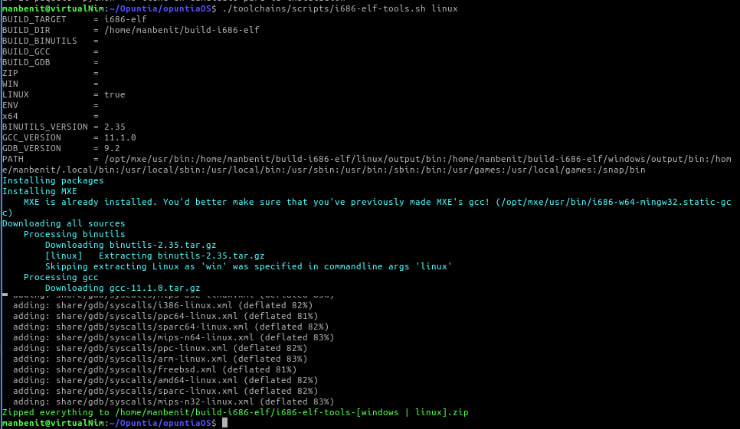
\includegraphics[scale=0.62]{toolchainx86.jpg}}
		\vspace{0.5cm}
		\subfloat[Resultado]{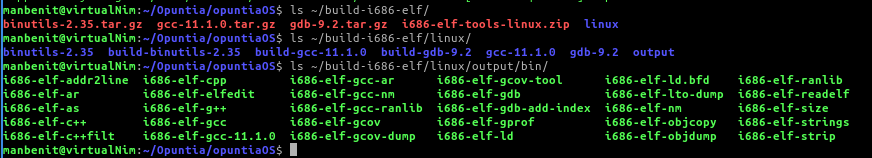
\includegraphics[scale=0.4]{toolchainx86_res.png}}
		\caption{
			Instalación del \textit{toolchain} para \texttt{x86}.
			\label{fig:toolchainx86}
		}
	\end{figure}

	
	
	Los binarios obtenidos de la instalación del \textit{toolchain} deben 
	agregarse a la variable de entorno del sistema (\texttt{PATH}) para
	su posterior uso en la construcción del sistema:
	\begin{center}
		\ttfamily
		export PATH=\$PATH:<directorio\_de\_contrucción>/linux/output/bin,
	\end{center}

	donde, \texttt{<directorio\_de\_contrucción>} es la ruta donde se 
	crea el \textit{toolchain}, por defecto se crea en \texttt{\$HOME}.
	
	
	
\newpage
\subsection{Instalación del \textit{toolchain} para ARM}
	Se deben asignar permisos de ejecución al \textit{script} de instalación por medio de 
	\begin{center}
		\ttfamily
		chmod 775 toolchains/scripts/arm-none-eabi-tools.sh,
	\end{center}

	este archivo se referencia en \texttt{docs/build.md}, sección \textit{GNU Toolchain for Linux (Ubuntu)}, del repositorio de \texttt{OpuntiaOS}.
	
	
	
	El \textit{script} se encarga de descargar y crear enlaces simbólicos a los binarios necesarios par ala compilación del sistema para \texttt{ARM}, sin embargo ocurren problemas debido a los nombres usados cuando se crean los enlaces simbólicos, además de hacer falta el \texttt{arm-none-eabi-objcopy}, necesario para la compilación, por lo que se recomienda modificar el \textit{script} como muestra la \autoref{fig:modifArmSsh}.
	\begin{figure}[ht]
		\centering
		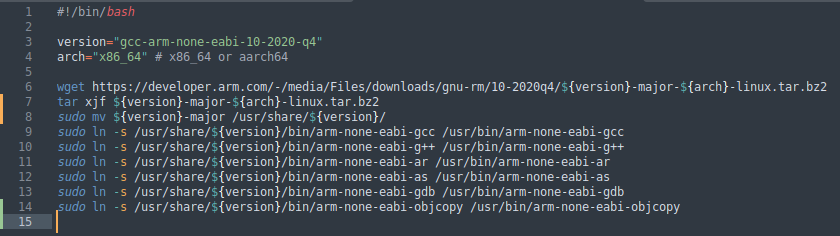
\includegraphics[scale=0.47]{modifArmSsh.png}
		\caption{
			Modificación del archivo \texttt{arm-none-eabi-tools.sh}.
			\label{fig:modifArmSsh}
		}
	\end{figure}
	
	\newpage
	
	Finalmente debe ejecutarse como indica el repositorio:
	\begin{center}
		\ttfamily
		./toolchains/scripts/arm-none-eabi-tools.sh,
	\end{center}
	cuya ejecución se muestra en la \autoref{fig:toolchainArm}.
	\begin{figure}[ht]
		\centering
		\subfloat[Proceso]{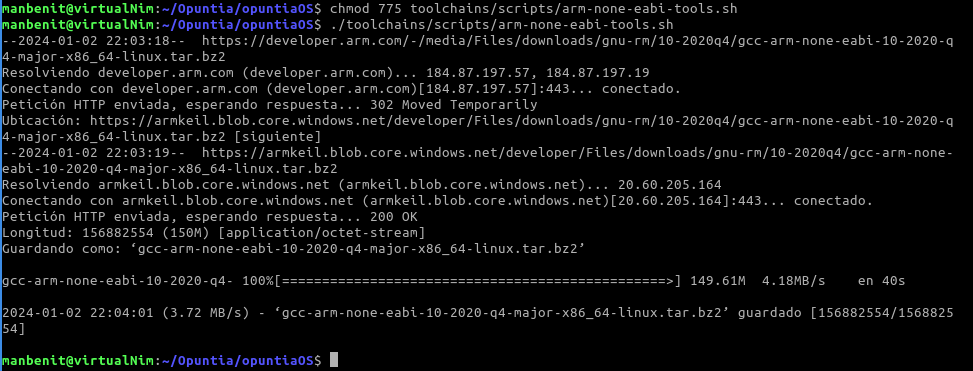
\includegraphics[scale=0.4]{toolchainArm.png}}
		\vspace{0.5cm}
		\subfloat[Resultado]{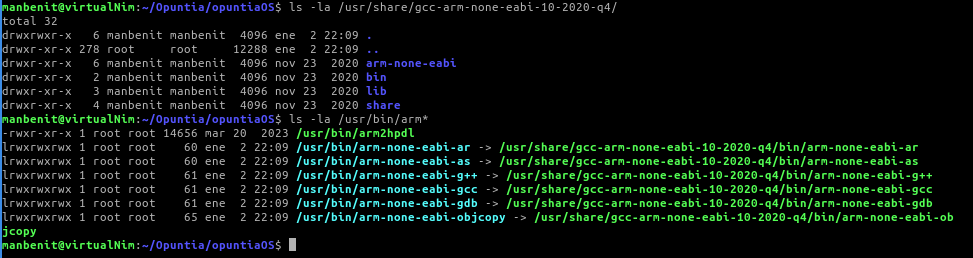
\includegraphics[scale=0.4]{toolchainArm_res.png}}
		\caption{
			Instalación del \textit{toolchain} para \texttt{ARM}.
			\label{fig:toolchainArm}
		}
	\end{figure}
	


	\clearpage
	\newpage \section{Procedimiento de compilación}
La compilación de \texttt{OpuntiaOS} se llevó a cabo en la distribución 
\texttt{Ubuntu 22.04.3 LTS}.



Para comenzar con la construcción del sistema es necesario haber realizado las
instalaciones mencionadas en la \autoref{sec:reqPrevios}, según la arquitectura.
	

\subsection{ARM}
	El procedimiento debe seguirse como lo menciona el archivo \texttt{docs/build.md} del repositorio, en la sección \textit{Building OS}, en este caso:
	\begin{center}
		\ttfamily
		./gn\_gen.sh --target\_arch arm.
	\end{center}
	
	A continuación se muestra el flujo de instrucciones utilizado para la construcción:
	\begin{figure}[ht]
		\centering
		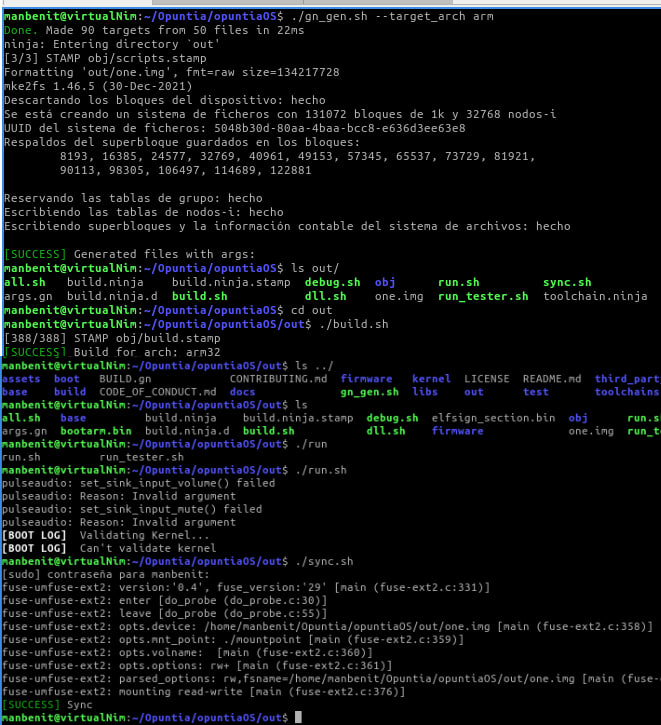
\includegraphics[scale=0.6]{buildArm.jpg}
		\caption{
			Construcción de la imagen de \texttt{OpuntiaOS} para \texttt{ARM}
			\label{fig:buildArm}
		}
	\end{figure}
	\begin{figure}[ht]
		\centering
		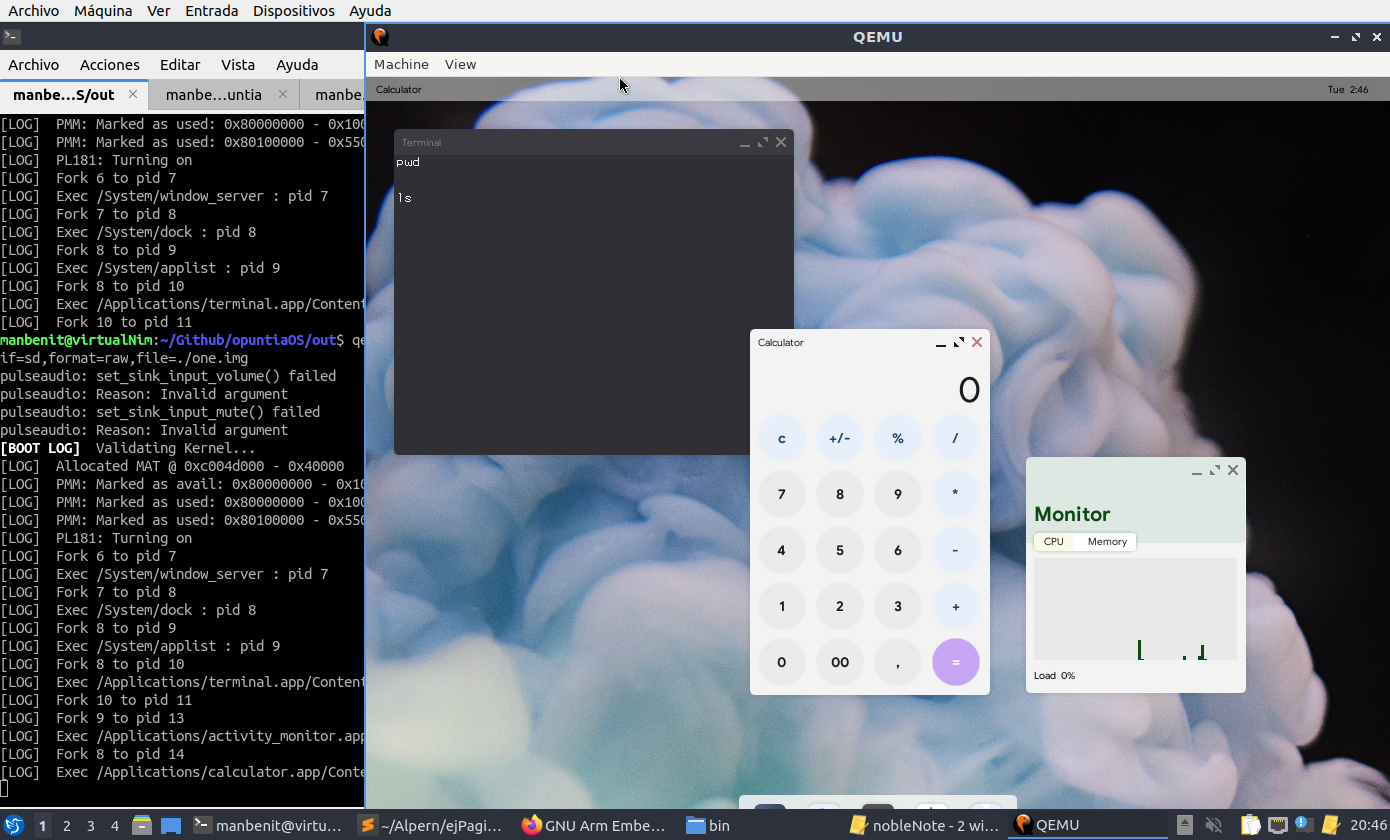
\includegraphics[scale=0.25]{primerARM.png}
		\caption{
			Arranque de la imagen de \texttt{OpuntiaOS} para \texttt{ARM}
			\label{fig:buildArm_res}
		}
	\end{figure}

	\textbf{NOTA}: Es importante ejecutar la sincronización (\texttt{sync.sh}) antes de 
	ejecutar el sistema (\texttt{run.sh}), si no se hace de esta forma, no terminan de sincronizarse los archivos con la imagen y el sistema se mostrará como muestra la \autoref{fig:armNoInit}.
	\begin{figure}[ht]
		\centering
		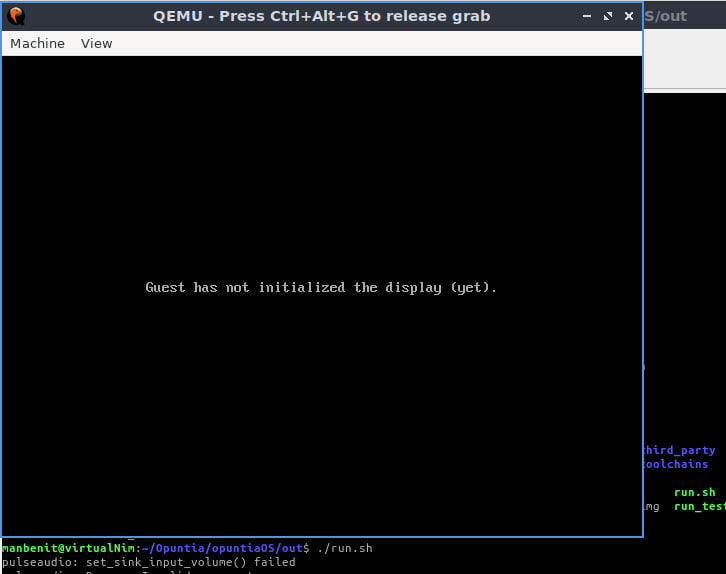
\includegraphics[scale=0.49]{armNoInit.jpg}
		\caption{
			Arranque de la imagen de \texttt{OpuntiaOS} para \texttt{ARM} si no se sincronizan los archivos.
			\label{fig:armNoInit}
		}
	\end{figure}





\newpage
\subsection{x86}
	El procedimiento debe seguirse como lo menciona el archivo \texttt{docs/build.md} del repositorio, en la sección \textit{Building OS}, en este caso:
	\begin{center}
		\ttfamily
		./gn\_gen.sh --target\_arch x86.
	\end{center}
	
	A continuación se muestra el flujo de instrucciones utilizado para la construcción:
	\begin{figure}[ht]
		\centering
		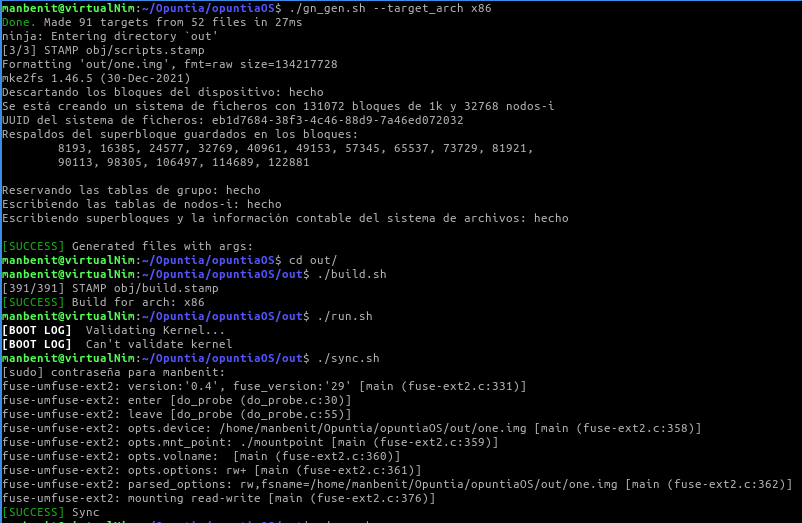
\includegraphics[scale=0.4]{buildx86.png}
		\caption{
			Construcción de la imagen de \texttt{OpuntiaOS} para \texttt{x86}
			\label{fig:buildx86}
		}
	\end{figure}
	\begin{figure}[ht]
		\centering
		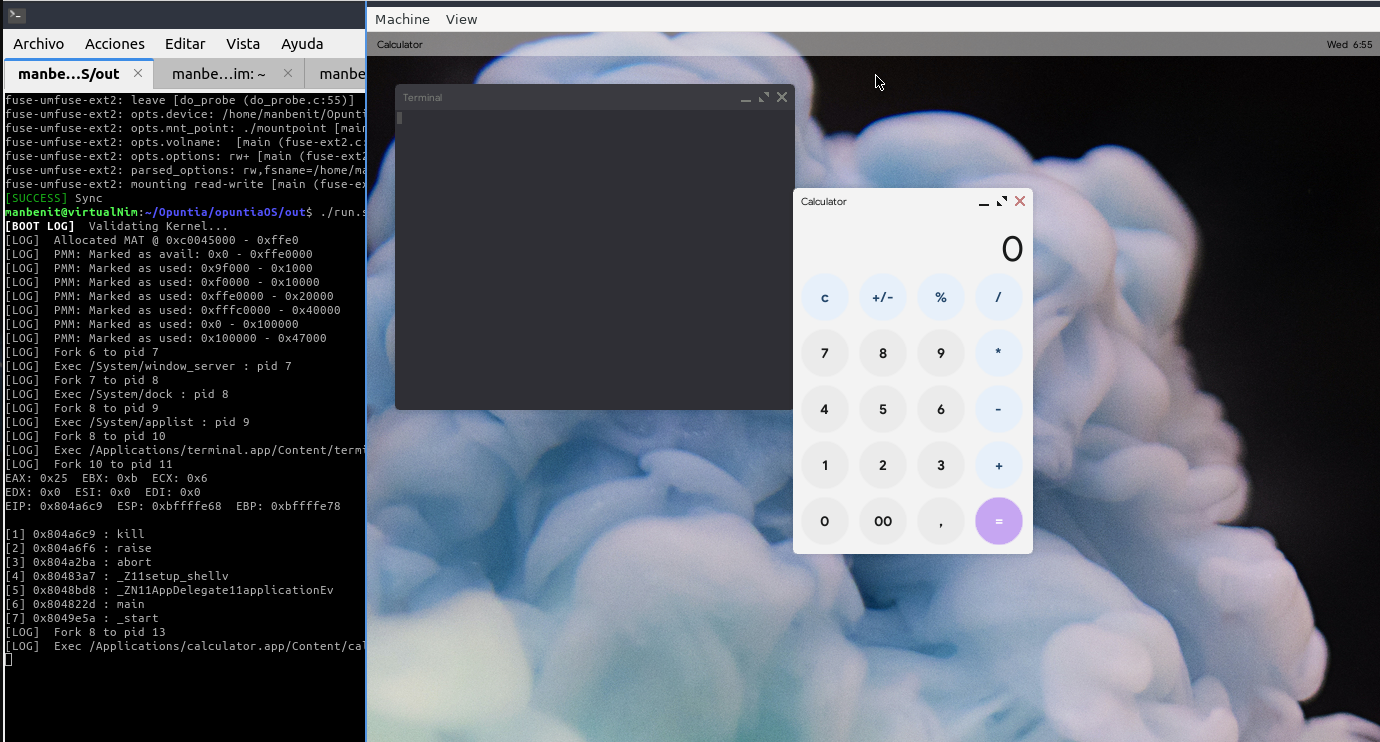
\includegraphics[scale=0.25]{primerx86.png}
		\caption{
			Arranque de la imagen de \texttt{OpuntiaOS} para \texttt{x86}
			\label{fig:buildx86_res}
		}
	\end{figure}
	
	\textbf{NOTA}: Es importante ejecutar la sincronización (\texttt{sync.sh}) antes de 
	ejecutar el sistema (\texttt{run.sh}), si no se hace de esta forma, no terminan de sincronizarse los archivos con la imagen y el sistema se mostrará como muestra la \autoref{fig:x86NoInit}.
	\begin{figure}[ht]
		\centering
		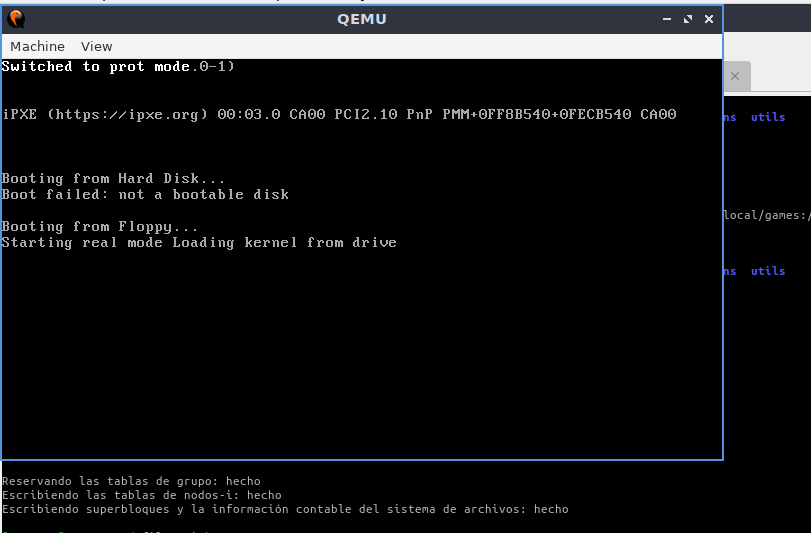
\includegraphics[scale=0.45]{x86NoInit.png}
		\caption{
			Arranque de la imagen de \texttt{OpuntiaOS} para \texttt{x86} si no se sincronizan los archivos.
			\label{fig:x86NoInit}
		}
	\end{figure}


















 \clearpage
	\newpage \section{Analisis}

\begin{comment}
	Los archivos build.ninja los utiliza el ninja como si fuera el Makefile.
	Los archivos BUILD.gn los usa gn [gen] como si fuera el Makefile.
	
\end{comment}


\subsection{Construcción del sistema}
	Cada directorio relacionado con la construcción contiene un archivo \texttt{BUILD.gn} o algún archivo de inclusión \texttt{.gni} y gracias al funcionamiento, descrito en la \autoref{ssec:gn}, se construye \texttt{OpuntiaOS} de manera ordenada.

	
	
	El archivo \texttt{gn\_gen.sh} es el encargado de generar los archivos necesarios para comenzar la construcción del sistema dentro del directorio \texttt{out}, esto gracias a \texttt{GN}, ejecutándose como se observa en la \autoref{fig:buildArm} y \autoref{fig:buildx86}.
	
	
	
	La primera ejecución relevante está en la línea:
	\begin{center}
		\ttfamily
		gn gen \$OUTDIR --args=\$GNARGS,
	\end{center}
	
	donde \texttt{OUTDIR} es \texttt{out} y \texttt{GNARGS} es, en el caso de la \autoref{fig:buildArm} y \autoref{fig:buildx86}, la arquitectura que se va a construir, entonces toma el valor \texttt{target\_arch=''arm''} o \texttt{target\_arch=''x86''}, según corresponda.
	
	
	
	Este argumento es transmitido a través de todos los archivos \texttt{BUILD.gn} de los diferentes directorios, principalmente se lee esta condición en los archivos de construcción \texttt{build/boot/BUILD.gn} y \texttt{build/config/BUILDCONFIG.gn}, así como en los archivos de inclusión \texttt{toolchains/COMPILERS.gni} y \\ \texttt{build/userland/USERLAND\_FLAGS.gni}.
	
	\begin{figure}[ht]
		\centering
		\subfloat[\texttt{ARM}]{
			\includegraphics[scale=0.3]{outPrebuild_ARM.png}
		}
		\hspace*{0.3cm}
		\subfloat[\texttt{x86}]{
			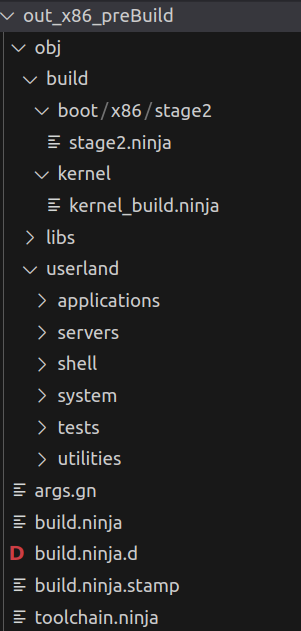
\includegraphics[scale=0.3]{outPrebuild_x86.png}
		}
		\caption{
			Árbol de carpetas del directorio \texttt{obj} creado previo a
			la construcción del sistema.
			\label{fig:outPrebuild}
		}
	\end{figure}

	
	\clearpage
	En este punto se genera un directorio que posteriormente es eliminado y contiene las definiciones \texttt{ninja} para la construcción de \textit{scripts} como \texttt{all.sh}, \texttt{build.sh}, \texttt{sync.sh} y \texttt{run.sh}, así como la compilación de los archivos de \textit{boot}, mismos cuyo código se encuentra en los directorios mostrados en la \autoref{fig:implBootloader}.
	
	
	
	La estructura de el directorio \texttt{out/obj/} se muestra en la \autoref{fig:outPrebuild}, donde puede observarse la diferencia en la estructura de construcción del \textit{kernel}.
	
	
	
	Por otro lado, en la \autoref{fig:compileLink} se observa la diferencia en los archivos construídos y su enlace, por medio del \texttt{boot\_link.ld} que se construye por medio de \texttt{GN}, similar a lo que se vio en el curso en los \textit{kernel} de Molloy, Bran's y Dennix.

	\begin{figure}[ht]
		\centering
		\subfloat[\texttt{ARM}]{
			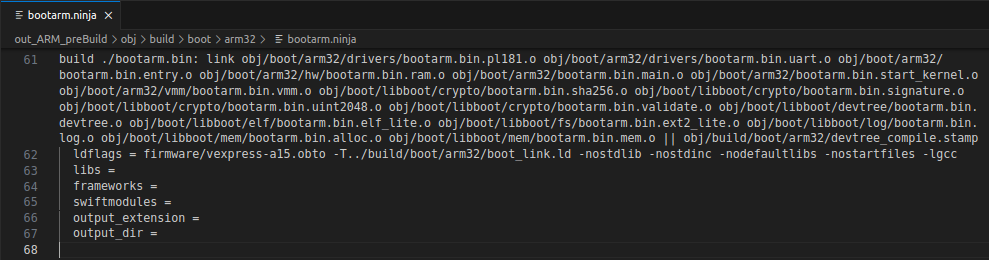
\includegraphics[scale=0.4]{compileLink_ARM.png}
		}
		\vspace*{0.3cm}
		\subfloat[\texttt{x86}]{
			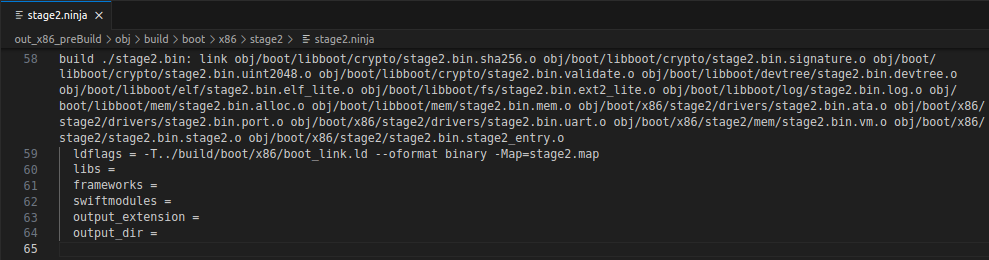
\includegraphics[scale=0.4]{compileLink_x86.png}
		}
		\caption{
			Instrucción de enlace de los archivos objeto generados del código fuente, similar a los archivos \texttt{Makefile} de los \textit{kernel} del curso.
			\label{fig:compileLink}
		}
	\end{figure}
	
	
	

\newpage
\subsection{Implementación del \textit{bootloader} \label{ssec:implBootloader}}
	Durante los temas vistos en el curso de Sistemas Operativos se vio que, 
	cuando se construye un sistema, una parte vital para el arranque es que el \textit{bootloader} otorgue control a dicho sistema (\autoref{fig:arranqueSO}), en el caso de \texttt{OpuntiaOS}, se tiene un manejo de la construcción del arranque con archivos \texttt{ninja}.
	\begin{figure}[ht]
		\centering
		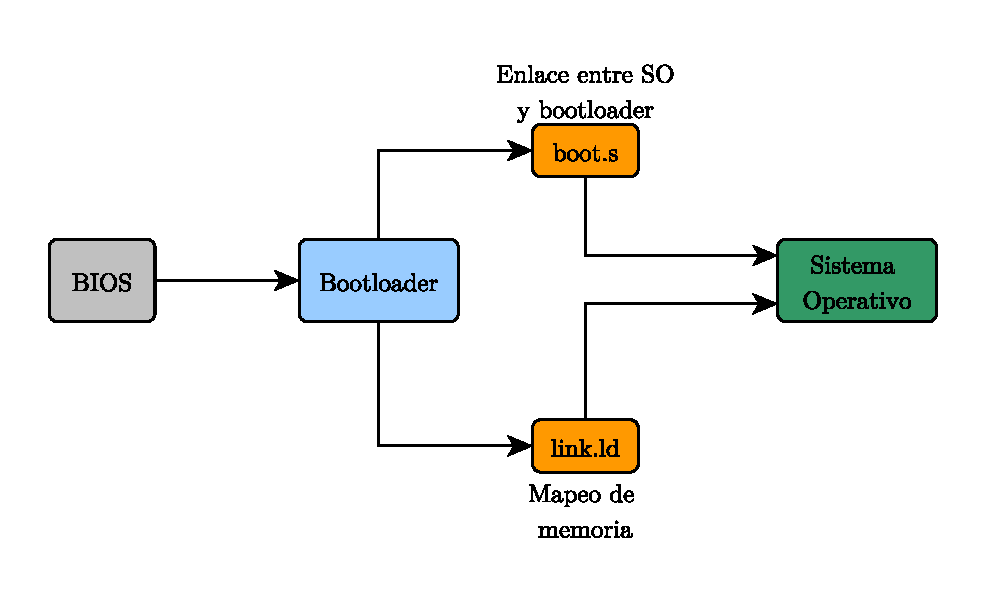
\includegraphics[scale=0.8]{arranqueSO.eps}
		\caption{
			Proceso de arranque de un sistema operativo.
			\label{fig:arranqueSO}
		}
	\end{figure}
	
	

	Lo primero de lo que es posible percatarse al analizar la implementación del \textit{bootloader} es que la estructura de carpetas y archivos es distinta para \texttt{ARM} y \texttt{x86}.
	\begin{figure}[ht]
		\centering
		\subfloat[\texttt{ARM} \label{sfig:implBloaderArm}]{
			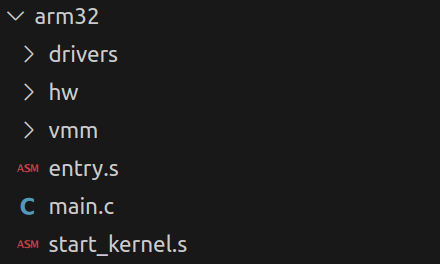
\includegraphics[scale=0.4]{estrucDir_ARM.png}
		}
		\hspace*{0.3cm}
		\subfloat[\texttt{x86} \label{sfig:implBloaderx86}]{
			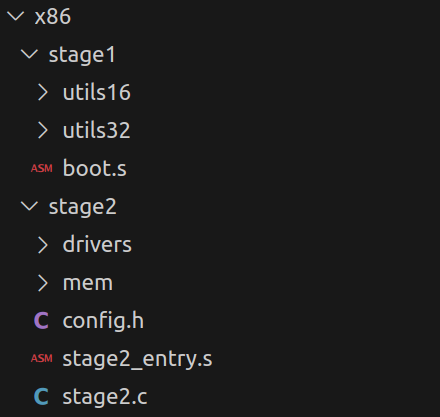
\includegraphics[scale=0.4]{estrucDir_x86.png}
		}
		\caption{
			Árbol de carpetas de implementación del \textit{bootloader}.
			\label{fig:implBootloader}
		}
	\end{figure}

	
	
	Por otra parte, se tiene el código de enlace (en el curso \texttt{link.ld}):
	\begin{itemize} \setlength\itemsep{0pt}
		\item \texttt{build/boot/x86/boot\_link.ld} para \texttt{x86},
		\item \texttt{build/boot/arm32/boot\_link.ld} para \texttt{ARM},
	\end{itemize}
	
	mismos que se llaman con ninja (ver \autoref{fig:compileLink}) y cabe mencionar que en el directorio \texttt{boot} se maneja la misma estructura que en la \autoref{fig:implBootloader}, pero solo con los archivos de construcción y el enlace.
	
	
	
	\subsubsection{En \texttt{x86}}
	En el caso de \texttt{OpuntiaOS} para \texttt{x86}, se manejan 2 archivos de etapa para el arranque del sistema en lugar de 1, es decir, no se generará el archivo \texttt{stage2\_eltorito}, si no que se generarán 2 archivos de carga de \textit{kernel}.
	\begin{figure}[ht]
		\centering
		\subfloat[Directorio \texttt{stage1} \label{sfig:x86Boot_stage1}]{
			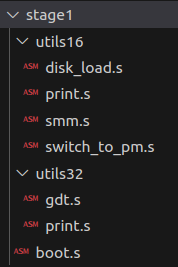
\includegraphics[scale=0.5]{x86_stage1_code.png}
		}
		\hspace*{1cm}
		\subfloat[Directorio \texttt{stage2} \label{sfig:x86Boot_stage2}]{
			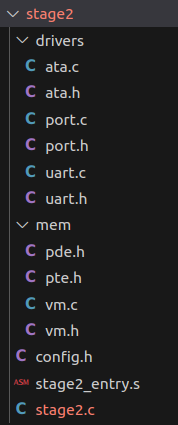
\includegraphics[scale=0.5]{x86_stage2_code.png}
		}
		\caption{
			Directorio de implementación del \textit{bootloader} para \texttt{x86}.
			\label{fig:x86Boot}
		}
	\end{figure}
	
	Como se aprecia en la \autoref{sfig:x86Boot_stage1}, la primera etapa de carga contiene solo código ensamblador, es to es porque \texttt{stage1} se carga desde la BIOS y es la encargado de realizar la primera carga del \textit{kernel}, se puede decir que el archivo más importante es \texttt{boot.s}, similar a los \textit{kernel} compilados en el curso.
	
	
	\clearpage
	Dentro del archivo \texttt{boot.s} se encuentra la carga del \textit{kernel} bajo instrucciones de 16 bits, que a su vez utiliza la carga del disco y mapeo de la memoria, y después la entrada a modo protegido, cuyas instrucciones deben considerarse de 32 bits y en este mismo tamaño de instrucciones se encuentra la definición de la GDT.
	\begin{figure}[ht]
		\centering
		\subfloat[Inclusión de utilidades para 16 y 32 bits. \label{sfig:x86_boots_include}]{
			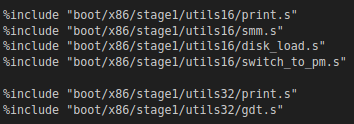
\includegraphics[scale=0.55]{x86_boots_include.png}
		}
		\vspace*{0.3cm}
		\subfloat[Código de 16 bits \label{sfig:x86_boots_16bits}]{
			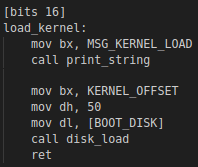
\includegraphics[scale=0.55]{x86_boots_16bits.png}
		}
		\hspace*{1cm}
		\subfloat[Código de 32 bits \label{sfig:x86_boots_32bits}]{
			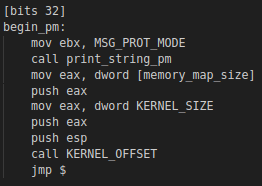
\includegraphics[scale=0.55]{x86_boots_32bits.png}
		}
		\caption{
			Código del archivo \texttt{boot.s} para la arquitectura \texttt{x86}.
			\label{fig:x86_boots}
		}
	\end{figure}

	Como se puede observar en la \autoref{fig:x86_boots}, se utilizan los registros de 16 bits además de los de 32, esto es debido a la retrocompatibilidad de la arquitectura \texttt{x86}.
	
	
	Por otro lado, en el \texttt{stage2} se tienen implementados lo siguientes controladores:
	\begin{itemize} \setlength\itemsep{0pt}
		\item Inicializador del disco de arranque (\texttt{ata.c} y \texttt{ata.h}).
		\item Lectura y escritura de puertos bajo 8, 16 y 32 bits (\texttt{port.c} y \texttt{port.h}).
		\item Inicialización y escritura de la interfaz UART (\texttt{uart.c} y \texttt{uart.h}).
	\end{itemize}
	
	
	
	Y también está la implementación del manejador de memoria:
	\begin{itemize} \setlength\itemsep{0pt}
		\item Definición de los descriptores de página (\texttt{pte.h}).
		\item Definición de los descriptores de tablas (\texttt{pde.h}).
		\item Memoria virtual del sistema utilizando paginación (\texttt{vm.c} y \texttt{vm.h}), y por lo tanto, los descriptores de tablas y de páginas de los 2 puntos anteriores.
	\end{itemize}

	
	
	Esta etapa es la que se encarga de cargar el \textit{kernel} a la memoria, esto se realiza preparando el disco de arranque por medio del archivo \texttt{stage2\_entry.s}.
	
	
	
	Esto lo hace inicializando la pila del procesador con ayuda del archivo enlazador para dar paso al \textit{kernel}, luego el encargado de realizar el proceso principal de la segunda etapa es \texttt{stage2.c}, que contiene el código para iniciar la memoria de arranque, preparar el disco y el sistema de archivos, validar el \textit{kernel} encontrado, cargar el \textit{kernel} a la memoria e iniciar la paginación de la memoria.

	
	
	
	\subsubsection{En \texttt{ARM}}
	En el caso de \texttt{OpuntiaOs} para \texttt{ARM} se debe entender cómo funciona el arranque de dicha arquitectura.
	
	
	
	\texttt{ARM} es una arquitectura que se utiliza para los SoC (Sistemas en Chip) y sigue un proceso de arranque similar al de una PC con \texttt{x86}, con la diferencia de que la información encesaria para arrancar no se carga desde un disco duro, si no desde una tarjeta \texttt{SD} y su \textit{bootloader} no es \texttt{GRUB}, si no que es \texttt{U-boot} \cite{vargas_risc}.

	
	
	Una de las principales diferencias a nivel de código es que la dirección de arranque de \textit{kernel} no comienza en la dirección \texttt{0x80000000} como en \texttt{x86}, si no que lo hace en la \texttt{0x00000000}.
	
	
	
	El \textit{bootloader} de \texttt{ARM} trabaja en 2 etapas, la primera que trabaja en modo supervisor, que se encarga de acceder a los recursos del sistema y poder ejecutar el \textit{kernel} del sistema, siendo también el modo donde se ejecuta el sistema operativo en sí; luego está la etapa de modo usuario, donde se restringe el acceso a \textit{hardware}, se ejecutan solo algunas instrucciones a nivel ensamblador y se tienen todas las aplicaciones que el usuario necesita y a las que puede acceder.
	
	
	
	Gracias al modo de arranque en modo supervisor de esta arquitectura, su código de arranque es más sencillo, no solo porque tiene un acceso más directo al \textit{hardware} en el mismo nivel donde trabaja el sistema operativo, si no que se basa en instrucciones \texttt{RISC}, lo cual baja complejidad al código utilizado para su manipulación.
	\begin{figure}[ht]
		\centering
		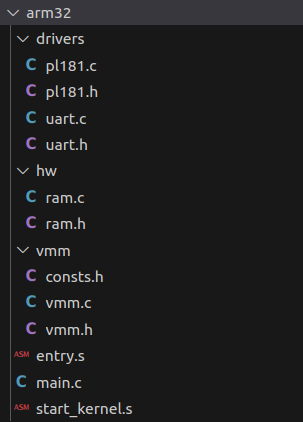
\includegraphics[scale=0.5]{arm_boot_code.png}
		\caption{
			Directorio de implementación del \textit{bootloader} para \texttt{ARM}.
			\label{fig:arm_boot_code}
		}
	\end{figure}
	
	\newpage
	
	En esta arquitectura las instrucciones son de 32 bits y los archivos principales del \textit{bootloader} son:
	\begin{itemize} \setlength\itemsep{0pt}
		\item \texttt{entry.s}: Contiene el código que se ejecuta en primer lugar cuando se enciende la máquina, se encarga de iniciar la pila y, como los diferentes sistemas en chip pueden tener uno o varios procesadores, se encarga de recorrer los id de cada procesador para iniciar cada pila adecuadamente .
		\item \texttt{start\_kernel.s}: Este código inicializa las estructuras de datos del \textit{kernel} y configura el sistema operativo, por medio de la llamada al archivo principal de configuración \texttt{main.c} luego de realizar esto, comienza la ejecución del \textit{kernel}.
	\end{itemize}
	\begin{figure}[ht]
		\centering
		\subfloat[]{
			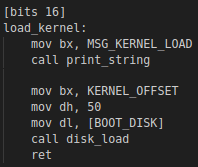
\includegraphics[scale=0.55]{x86_boots_16bits.png}
		}
		\hspace*{1cm}
		\subfloat[]{
			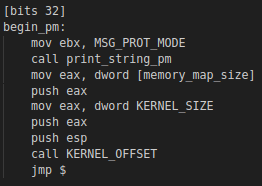
\includegraphics[scale=0.55]{x86_boots_32bits.png}
		}
		\caption{
			Código del archivo \texttt{start\_kernel.s} para la arquitectura \texttt{ARM}.
			\label{fig:arm_startkernels}
		}
	\end{figure}

	
	\clearpage
	Por otro lado, se tienen implementados los siguientes archivos:
	\begin{itemize} \setlength\itemsep{0pt}
		\item \textbf{Controladores}
		\begin{itemize} \setlength\itemsep{0pt}
			\item Mapeo y lectura de la tarjeta SD de donde se va a cargar el sistema operativo, debe su nombre a la celda 
			PL181\footnote{
				La tarjeta multimedia \texttt{PL180/181} es un periférico \texttt{ARM} para tarjetas multimedia (MMC) y tarjetas digitales seguras (SD) en formato de E/S, asignadas en memoria compatible con el bus periférico avanzado (APB) de \texttt{ARM} \cite{pl181}.
			}
			donde se introducen dichas tarjetas (\texttt{pl181.c} y \texttt{pl181.h}).
			
			\item Inicialización y lectura de la interfaz UART (\texttt{uart.c} y \texttt{uart.h}).
		\end{itemize}
	
		\item \textbf{Manejo de \textit{hardware}}
		\begin{itemize} \setlength\itemsep{0pt}
			\item Lector de tamaño de la memoria RAM instalada en el dispositivo (\texttt{ram.c} y \texttt{ram.h}).
		\end{itemize}
	
		\item \textbf{Manejo de memoria}
		\begin{itemize} \setlength\itemsep{0pt}
			\item Definición de constantes para el manejo de la memoria virtual (\texttt{consts.hh}).
			
			\item Memoria virtual del sistema utilizando paginación,para ello definiendo las estructuras para los descriptores de tablas y de páginas (\texttt{vmm.c} y \texttt{vmm.h}), utilizando las constantes definidas del punto anterior.
		\end{itemize}
	\end{itemize}

	
	\newpage
	La implementación del \textit{bootloader} de ambas arquitecturas utiliza, en común, los archivos del directorio \texttt{libboot}, que contiene las estructuras de datos y algunas implementaciones para hacer la validación del sistema (firma, seguridad, sistema de archivos \texttt{ext2}, etc.) y que éste arranque de forma correcta y segura.
	\begin{figure}[ht]
		\centering
		\subfloat[]{
			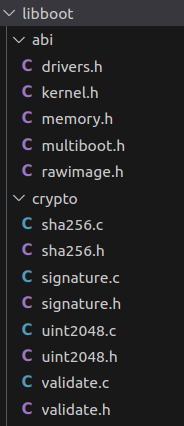
\includegraphics[scale=0.5]{libboot_p1.png}
		}
		\hspace*{1cm}
		\subfloat[]{
			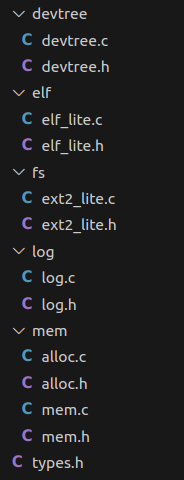
\includegraphics[scale=0.5]{libboot_p2.png}
		}
		\caption{
			Archivos del directorio \texttt{libboot}, común para las arquitecturas analizadas (\texttt{ARM} y \texttt{x86}).
			\label{fig:libboot}
		}
	\end{figure}

	
	
	Otro directorio que implementan en común las 2 arquitecturas es \texttt{libs}, que contiene, entre otras cosas, manejadores de memoria, definiciones para funcionamiento de la interfás gráfica y las definiciones de funciones para lenguaje \texttt{C}, tales como \texttt{malloc, execve, fork}, etc.
	\begin{figure}[ht]
		\centering
		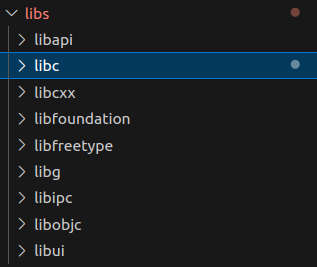
\includegraphics[scale=0.5]{libs.png}
		\caption{
			Directorio \texttt{libs}.
			\label{fig:libs}
		}
	\end{figure}
	

\newpage
\subsection{Comparativa \texttt{ARM} y \texttt{x86}}
	En principio, el \textit{bootloader} de ambas arquitecturas presenta similitudes en cuanto a las tareas básicas del sistema.
	
	
	
	Una similitud se encuentra en la manera en que funcionan, porque ambos se encargan de realizar las tareas básicas de arranque del sistema, como:
	\begin{itemize} \setlength\itemsep{0pt}
		\item \textbf{Inicialización del hardware}: Detectar y configurar la memoria, el CPU, los dispositivos de almacenamiento y otros componentes del sistema.
		
		\item \textbf{Carga del sistema operativo}: Buscar y cargar el \textit{kernel} del sistema operativo en la memoria.
		
		\item \textbf{Transferencia de control}: Transferir el control al \textit{kernel} del sistema operativo para que se inicie el sistema.
	\end{itemize}

	Y otro aspecto similar es la estructura que tienen, porque ambos tienen una fase de arranque temprano y una fase de arranque tardío.
	\begin{itemize} \setlength\itemsep{0pt}
		\item \textbf{Fase de arranque temprano}: Se ejecuta en \textbf{modo real} en \texttt{x86} y en \textbf{modo supervisor} en \texttt{ARM}. 
		
		
		
		En esta fase se hace una inicialización básica del \textit{hardware} y carga el \textit{kernel} del \textit{bootloader}.
		
		
		\item \textbf{Fase de arranque tardío}: Se ejecuta en \textbf{modo protegido} en \texttt{x86} y en \textbf{modo usuario} en \texttt{ARM}. 
		
		
		
		En esta fase se cargan los controladores adicionales, la configuración del sistema y la presentación de un menú de arranque.
	\end{itemize}
	
	
	
	Luego, de acuerdo con la información analizada en la \autoref{ssec:implBootloader}, es posible notar varias diferencias en la manera en que se arranca el sistema en las arquitecturas \texttt{ARM} y \texttt{x86}, en la \autoref{tab:bootldrCompArranque} se presenta una comparativa entre ellas.
	\begin{table}[ht]
		\centering
		\begin{tabular}{|
				>{\columncolor[HTML]{ECF4FF}}c |c|c|}
			\hline
			\multicolumn{1}{|l|}{\cellcolor[HTML]{000000}} & \cellcolor[HTML]{68CBD0}\textbf{x86} & \cellcolor[HTML]{68CBD0}\textbf{ARM}                                                    \\ \hline
			\textbf{Instrucciones}                         & Complejas, de 16 y 32 bits           & Reducidas, de 32 bits                                                                     \\ \hline
			\textbf{Modo de arranque}                      & En modo real                         & En modo supervisor                                                                      \\ \hline
			\textbf{Acceso a hardware}                     & Tiene acceso directo                 & \begin{tabular}[c]{@{}c@{}}Utiliza interfaces del \\ firmware del sistema\end{tabular} \\ \hline
			\textit{\textbf{Firmware}}                     & Utiliza BIOS                         & Utiliza U-Boot o UEFI                                                                   \\ \hline
			\textbf{Herramientas}                          & GRUB y LILO                          & U-Boot y UEFI                                                                           \\ \hline
		\end{tabular}
		\caption{
			Comparación del modo de arranque de \texttt{ARM} y \texttt{x86}.
			\label{tab:bootldrCompArranque}
		}
	\end{table}
	
	\newpage
	
	Durante el curso de sistemas operativos se abordo el tema del modo real y modo protegido de la arquitectura\texttt{x86}, siendo el primero cuando se tiene acceso directo a rutinas de la BIOS y el \textit{hardware} y el segundo cuando se restringe el acceso a privilegios del sistema usando GDT, IDT y memoria virtual por paginación.
	
	
	
	En \texttt{ARM} existen homólogos denominados ``modo supervisor'' y ``modo usuario'', que cumplen una función similar al modo real y protegido, respectivamente.
	
	
	Los modos supervisor y usuario de ARM se utilizan para:
	\begin{itemize} \setlength\itemsep{0pt}
		\item \textbf{Protección}
		\begin{itemize} \setlength\itemsep{0pt}
			\item \underline{Modo supervisor}: Permite el acceso a recursos sensibles como memoria, dispositivos de E/S e instrucciones privilegiadas. Se utiliza para ejecutar el \textit{kernel}, controladores de dispositivos y otras tareas críticas del sistema.
			
			\item \underline{Modo usuario}: Limita el acceso a recursos del sistema y solo permite ejecutar instrucciones no privilegiadas. Se usa para ejecutar aplicaciones de usuario, esto protege el sistema operativo y el \textit{hardware} de posibles errores o acciones maliciosas.
		\end{itemize}
	
		\item \textbf{Aislamiento}
		\begin{itemize} \setlength\itemsep{0pt}
			\item \underline{Modo supervisor}: Ofrece un entorno seguro para ejecutar el sistema operativo y las tareas críticas del sistema, sin interferencias de las aplicaciones de usuario.
			
			\item \underline{Modo usuario}: Proporciona un entorno aislado para ejecutar aplicaciones de usuario, evitando que puedan acceder a recursos del sistema que no necesitan.
		\end{itemize}
	
		\item \textbf{Rendimiento}
		\begin{itemize} \setlength\itemsep{0pt}
			\item \underline{Modo supervisor}: Permite un mayor rendimiento al ejecutar código privilegiado que necesita acceso directo al \textit{hardware}.
			
			\item \underline{Modo usuario}: Permite un uso más eficiente de la memoria al ejecutar código no privilegiado en un espacio de memoria separado.
		\end{itemize}
	\end{itemize}

	
	
	En consecuencia, es posible comparar la funcionalidad de los modos de arranque para ambas arquitecturas, lo cuál se muestra en la \autoref{tab:bootldrCompStage1} y \autoref{tab:bootldrCompStage2}.
	\begin{table}[ht]
		\centering
		\begin{tabular}{|
				>{\columncolor[HTML]{ECF4FF}}c |c|c|}
			\hline
			\multicolumn{1}{|l|}{\cellcolor[HTML]{000000}}                                 & \cellcolor[HTML]{68CBD0}\textbf{Modo real} & \cellcolor[HTML]{68CBD0}\textbf{Modo supervisor}                            \\ \hline
			\textbf{Nivel de privilegios}                                                  & Bajo                                       & Alto                                                                        \\ \hline
			\textbf{Acceso a memoria}                                                      & Segmentado                                 & Completo                                                                    \\ \hline
			\textbf{\begin{tabular}[c]{@{}c@{}}Acceso a \\ dispositivos E/S\end{tabular}}  & Limitado                                   & Completo                                                                    \\ \hline
			\textbf{\begin{tabular}[c]{@{}c@{}}Ejecución de \\ instrucciones\end{tabular}} & No privilegiadas                           & \begin{tabular}[c]{@{}c@{}}Privilegiadas y \\ no privilegiadas\end{tabular} \\ \hline
		\end{tabular}
		\caption{
			Comparación del modo real de \texttt{x86} y el modo supervisor de \texttt{ARM}.
			\label{tab:bootldrCompStage1}
		}
	\end{table}

	\begin{table}[ht]
		\centering
		\begin{tabular}{|
				>{\columncolor[HTML]{ECF4FF}}c |c|c|}
			\hline
			\multicolumn{1}{|l|}{\cellcolor[HTML]{000000}}                                 & \cellcolor[HTML]{68CBD0}\textbf{Modo protegido}                                & \cellcolor[HTML]{68CBD0}\textbf{Modo usuario}                                \\ \hline
			\textbf{Nivel de privilegios}                                                  & Alto                                                                           & Bajo                                                                         \\ \hline
			\textbf{Acceso a memoria}                                                      & \begin{tabular}[c]{@{}c@{}}Segmentado y \\ paginado\end{tabular}               & \begin{tabular}[c]{@{}c@{}}Limitado por \\ el segmento\end{tabular}          \\ \hline
			\textbf{\begin{tabular}[c]{@{}c@{}}Acceso a \\ dispositivos E/S\end{tabular}}  & \begin{tabular}[c]{@{}c@{}}Controlado por el \\ sistema operativo\end{tabular} & \begin{tabular}[c]{@{}c@{}}Limitado por el \\ sistema operativo\end{tabular} \\ \hline
			\textbf{\begin{tabular}[c]{@{}c@{}}Ejecución de \\ instrucciones\end{tabular}} & \begin{tabular}[c]{@{}c@{}}Privilegiadas y \\ no privilegiadas\end{tabular}    & \begin{tabular}[c]{@{}c@{}}No \\ privilegiadas\end{tabular}             \\ \hline
		\end{tabular}
		\caption{
			Comparación del modo protegido de \texttt{x86} y el modo usuario de \texttt{ARM}.
			\label{tab:bootldrCompStage2}
		}
	\end{table}
				
	\newpage
	
	En general, tanto los modos de \texttt{x86} como de \texttt{ARM} cumplen con las mismas funcione:
	\begin{itemize} \setlength\itemsep{0pt}
		\item Ambos pares de modos ofrecen diferentes niveles de acceso a los recursos del sistema.
		\item El modo con más privilegios se utiliza para ejecutar código crítico del sistema en espacio de \textit{kernel}, mientras que el menos privilegiado se utiliza para ejecutar aplicaciones en espacio de usuario.
	\end{itemize}	

	
	
	Sin embargo, basado en lo comparado en la \autoref{tab:bootldrCompStage1} y \autoref{tab:bootldrCompStage2}, así como en la \autoref{ssec:implBootloader}, se puede destacar lo siguiente:
	\begin{itemize} \setlength\itemsep{0pt}
		\item El modo supervisor es un modo de 32 bits, mientras que el modo real es un modo de 16 bits.
		
		\item El modo supervisor ofrece un mayor control sobre el \textit{hardware} y la memoria.
		
		\item El modo usuario ofrece un mayor aislamiento entre las aplicaciones.
		
		\item El modo protegido permite una gestión más eficiente de la memoria.
	\end{itemize}

	\newpage
	
	Finalmente se puede obtener una comparación entre el arranque del \textit{bootloader} de ambas arquitecturas.
	\begin{table}[ht]
		\centering
		\resizebox{\textwidth}{!}{ \begin{tabular}{|c|cc|}
			\hline
			\rowcolor[HTML]{68CBD0} 
			\multicolumn{1}{|l|}{\cellcolor[HTML]{000000}}                                & \multicolumn{1}{c|}{\cellcolor[HTML]{68CBD0}\textbf{x86}}                                                                                                                    & \textbf{ARM}                                                                                                                                                   \\ \hline
			\cellcolor[HTML]{ECF4FF}\textbf{Ubicación}                                    & \multicolumn{1}{c|}{\begin{tabular}[c]{@{}c@{}}MBR del disco \\ de arranque\end{tabular}}                                                                                    & \begin{tabular}[c]{@{}c@{}}Disco de arranque\\ (ej: tarjeta SD)\end{tabular}                                                                                   \\ \hline
			\cellcolor[HTML]{ECF4FF}\textbf{Modo de ejecución}                            & \multicolumn{1}{c|}{Modo real}                                                                                                                                               & Modo supervisor                                                                                                                                                \\ \hline
			\cellcolor[HTML]{ECF4FF}\textbf{Funciones}                                    & \multicolumn{1}{c|}{\begin{tabular}[c]{@{}c@{}}- Carga el \textit{kernel} del sistema operativo. \\ - Transfiere el control al \textit{kernel}. \\ - Ofrece un menú de arranque.\end{tabular}} & \begin{tabular}[c]{@{}c@{}}- Carga el \textit{kernel} del sistema operativo. \\ - Transfiere el control al \textit{kernel}. \\ - Puede ofrecer un menú de arranque.\end{tabular} \\ \hline
			\textbf{\begin{tabular}[c]{@{}c@{}}Diferencias más\\ relevantes\end{tabular}} & \multicolumn{1}{c|}{\begin{tabular}[c]{@{}c@{}}- Arranca en modo real. \\ - Código de 16 bits. \\ - Acceso directo al \textit{hardware}.\end{tabular}}                                & \begin{tabular}[c]{@{}c@{}}- Arranca en modo supervisor. \\ - Código de 32 bits (o 64 bits). \\ - Usa interfaces del \textit{firmware}.\end{tabular}                    \\ \hline
			\textbf{Similitudes}                                                          & \multicolumn{2}{c|}{\begin{tabular}[c]{@{}c@{}}- Carga el \textit{kernel} del sistema operativo. \\ - Transfiere el control al \textit{kernel}. \\ - Ofrece opciones de configuración.\end{tabular}}                                                                                                                                                            \\ \hline
			\cellcolor[HTML]{ECF4FF}\textbf{Ejemplos}                                     & \multicolumn{1}{c|}{GRUB, LILO}                                                                                                                                              & U-Boot, UEFI                                                                                                                                                   \\ \hline
		\end{tabular}}
		\caption{
			Comparación del funcionamiento del \textit{bootloader} de \texttt{ARM} y \texttt{x86}. 
			\label{tab:bootldrComparaGral}	
		}
	\end{table}
	

\clearpage
\subsection{Temas vistos en el curso de Sistemas Operativos}
	El código fuente del \textit{kernel} de \texttt{OpuntiaOS} se encuentra en el directorio \texttt{kernel} y está dividido en 2 directorios, \texttt{include} y \texttt{kernel}.
	
	
	
	Tal como muestra la \autoref{fig:kernel_code}, ambos directorios tienen, prácticamente, la misma estructura, pero el directorio \texttt{include} contiene archivo \texttt{.h} para definir las funciones y constantes necesarias para la compilación del \textit{kernel}, mientras que \texttt{kernel} contiene las implementaciones de estas cabeceras.
	\begin{figure}[ht]
		\centering
		\subfloat[Directorio \texttt{include} \label{sfig:kernel_code_include}]{
			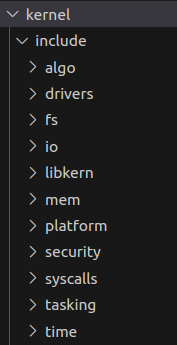
\includegraphics[scale=0.5]{kernel_code_include.png}
		}
		\hspace{3cm}
		\subfloat[Directorio \texttt{kernel} \label{sfig:kernel_code_kernel}]{
			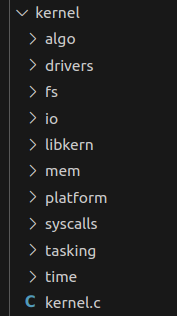
\includegraphics[scale=0.5]{kernel_code_kernel.png}
		}
		\caption{
			Directorio de implementación del \textit{kernel} de \texttt{OpuntiaOS}.
			\label{fig:kernel_code}
		}
	\end{figure}

	
	
	Una particularidad de esta estructura de carpetas es el directorio \texttt{platform}, el cual contiene las definiciones e implementaciones, respectivamente, que corresponden a cada una de las arquitecturas que soporta \texttt{OpuntiaOS}.
	
	
	
	A continuación se empatará el código visto en el curso con el contenido del código de \texttt{OpuntiaOS} siguiendo el orden del proyecto de James Molloy.
	
	
	
	\clearpage
	\subsubsection{Génesis}
		Archivos de Molloy: \texttt{boot.s, link.ld}.
		
		Para x86
		\begin{itemize} \setlength\itemsep{0pt}
			\item \texttt{build/boot/x86/boot\_link.ld}: El programa de carga se coloca en la dirección \texttt{0x1000}.
			\item \texttt{boot/x86/stage1/boot.s}: Carga del kernel.
			\item \texttt{boot/x86/stage2/stage2\_entry.s}: Inicialización de las estructuras del kernel.
		\end{itemize}
	
		NOTA: El archivo \texttt{boot/x86\_64/prekernel/mboot1.S} contiene una estructura mucho más similar al ensamblador proporcionado en el proyecto de Molloy, sin embargo el presente documento contempla la compilación en \texttt{x86} y no en \texttt{x86\_64}.
		
		
		Para ARM
		\begin{itemize} \setlength\itemsep{0pt}
			\item \texttt{build/boot/arm32/boot\_link.ld}: El programa de carga se coloca en la dirección \texttt{0x80010000}.
			\item \texttt{boot/arm32/entry.s}: Carga del kernel.
			\item \texttt{boot/arm32/start\_kernel.s}: Inicialización de las estructuras del kernel.
		\end{itemize}
		
		
		
	
	\subsubsection{La pantalla}
		En el código de Molloy se implementan los tipos de dato que se utilizan en todo el proyecto en el archivo \texttt{common.h} y \texttt{common.c}, en \texttt{OpuntiaOS} se usan:
		\begin{itemize} \setlength\itemsep{0pt}
			\item \texttt{boot/libboot/types.h}: Los tipos de dato que utiliza el \textit{bootloader}.
			
			\item \texttt{kernel/include/libkern/types.h}: Los tipos de dato que utiliza el código del \textit{kernel} para poder ser compilado.
			
			\item \texttt{libs/libc/include/sys/types.h}: Los tipos de dato que se utilizan como parte de la implementación, en lenguaje \texttt{C}, del sistema.
		\end{itemize}
	
		Estos archivos son utilizados por ambas arquitecturas.
	
		
		
		Luego, Molloy implementa el manejo de la pantalla con los archivos \texttt{monitor.h} y \texttt{monitor.c}; como \texttt{OpuntiaOS} es un sistema con ambiente gráfico, entonces se implementan los siguientes manejadores de pantalla:
		
		la pantalla tal como se vio en el curso, colocando la dirección de memoria de arranque de pantalla, pero se incluye el manejo de el ambiente gráfico y soporte de ventanas del sistema:
		\begin{itemize} \setlength\itemsep{0pt}
			\item \textbf{Inicialización y control}: Similar al proyecto en clase, se utiliza la pantalla con sus direcciones de memoria y manipulación de caracteres, se usan las definiciones en
			\texttt{kernel/include/drivers/debug/screen.h}\\
			y las implementaciones en 
			\texttt{kernel/kernel/drivers/debug/screen.c}.
			
			\item \textbf{Interfaz gráfica}: Se define el soporte para la interfaz gráfica del sistema en 
			\texttt{libs/libui/include/libui/Screen.h} y se utiliza en \\
			\texttt{libs/libui/src/Window.cpp}. \\
			Como puede notarse, esta implementación es en \texttt{C++}.
			
			
			\item \textbf{Ventanas del sistema}: Se define el manejo de ventanas en el archivo \texttt{userland/servers/window\_server/src/devices/Screen.h}, que se implementa en \texttt{userland/servers/window\_server/src/devices/Screen.cpp}, siendo desarrollado en \texttt{C++} y usándose en varios archivos dentro de\\ \texttt{userland/servers/window\_server/src/Components}.
		\end{itemize}
	
		Estos archivos son utilizados por ambas arquitecturas.
	
	
	
	
	
	\subsubsection{GDT e IDT}
		Archivos de Molloy: \texttt{gdt.s, interrupt.s, descriptor\_tables.h, descriptor\_tables.c, isr.h, isr.c}.
		
		Para x86:
		\begin{itemize} \setlength\itemsep{0pt}
			\item Ensambladores
			\begin{itemize} \setlength\itemsep{0pt}
				\item \texttt{boot/x86/stage1/utils32/gdt.s}
				\item \texttt{kernel/kernel/platform/x86/i386/interrupts/interrupts.s}
			\end{itemize}	
		
			\item Descriptor de la GDT
			\begin{itemize} \setlength\itemsep{0pt}
				\item \texttt{kernel/include/platform/x86/gdt.h}
				\item \texttt{kernel/kernel/platform/x86/gdt.c}
			\end{itemize}	
		
			\item Descriptor de la IDT
			\begin{itemize} \setlength\itemsep{0pt}
				\item \texttt{kernel/include/platform/x86/idt.h}
				\item \texttt{kernel/kernel/platform/x86/interrupts/idt.c}
			\end{itemize}
			
			\item Parte donde se inicia la GDT e IDT
			\begin{itemize} \setlength\itemsep{0pt}
				\item \texttt{kernel/include/platform/x86/init.h}
				\item \texttt{kernel/kernel/platform/x86/init.c}
			\end{itemize}	
			
			\item Manejador de IRQ
			\begin{itemize} \setlength\itemsep{0pt}
				\item \texttt{kernel/include/platform/x86/irq\_handler.h}
				\item \texttt{kernel/kernel/platform/x86/interrupts/irq\_handler.c}
			\end{itemize}	
			
			\item Rutinas de interrupciones (ISR)
			\begin{itemize} \setlength\itemsep{0pt}
				\item \texttt{kernel/include/platform/x86/isr\_handler.h}
				\item \texttt{kernel/kernel/platform/x86/interrupts/isr\_handler.c}
			\end{itemize}	
		\end{itemize}
	
		La arquitectura ARM no utiliza una GDT ni una IDT de la misma manera que lo hace la x86.
		
		%En la arquitectura x86, la GDT se utiliza para almacenar descripciones de segmentos de memoria y la IDT se utiliza para gestionar las interrupciones. Estos conceptos están relacionados con la gestión de memoria y la manipulación de interrupciones en la arquitectura x86.
		
		ARM utiliza un modelo de segmentación de memoria plano (\textit{Flat Memory Model}), lo que significa que no hay segmentos de memoria separados como en x86. En lugar de la IDT, ARM utiliza vectores de interrupción y excepción.
		
		
	
		Para ARM:
		\begin{itemize} \setlength\itemsep{0pt}
			\item Ensambladores
			\begin{itemize} \setlength\itemsep{0pt}
				\item \texttt{kernel/kernel/platform/arm32/interrupts/interrupts.s}
			\end{itemize}
		
			\item Descriptor de la tabla genérica de interrupciones
			\begin{itemize} \setlength\itemsep{0pt}
				\item \texttt{kernel/include/drivers/irq/arm/gicv2.h}
				\item \texttt{kernel/kernel/drivers/irq/arm/gicv2.c}
			\end{itemize}
		
			\item Configuración de interrupciones y excepciones
			\begin{itemize} \setlength\itemsep{0pt}
				\item \texttt{kernel/include/platform/arm32/interrupts.h}
				\item \texttt{kernel/kernel/platform/arm32/interrupts/handlers.c}
			\end{itemize}
		
			\item Parte del código donde se inicia el controlador genérico de interrupciones (GIC) y las interrupciones.
			\begin{itemize} \setlength\itemsep{0pt}
				\item \texttt{kernel/include/platform/arm32/init.h}
				\item \texttt{kernel/kernel/platform/arm32/init.c}
			\end{itemize}	
		\end{itemize}
	
	
		
	
	
	\subsubsection{IRQ y PIT}
		Archivos de Molloy: \texttt{timer.h, timer.c}.
		
		La PIT)es un componente se utiliza para generar interrupciones periódicas, como las interrupciones del sistema operativo que pueden ser usadas para mantener el tiempo del sistema, gestionar tareas programadas, etc.
		
		En la arquitectura ARM no hay un PIT estándar, por otro lado, pueden usar temporizadores o contadores específicos que son parte del diseño del sistema embebido o del SoC, que pueden variar entre diferentes dispositivos.
		
		Para ambas arquitecturas se implementa un Administrador principal de \textit{ticks}:\\
		\texttt{kernel/include/time/time\_manager.h} \\
		\texttt{kernel/kernel/time/time\_manager.c}
		
		Para x86
		\begin{itemize} \setlength\itemsep{0pt}
			\item \texttt{kernel/include/drivers/timer/x86/pit.h}
			\item \texttt{kernel/kernel/drivers/timer/x86/pit.c}
			
		\end{itemize}
	
		Para ARM:
		En el caso de OpuntiaOS, se implementa un temporizador enfocado en el temporizador SP804
		\begin{itemize} \setlength\itemsep{0pt}
			\item \texttt{kernel/kernel/drivers/timer/arm/sp804.c}
			\item \texttt{kernel/include/drivers/timer/arm/sp804.h}
		\end{itemize}
		
	
		

	
	\subsubsection{Paginación}
		Archivos de Molloy: \texttt{paging.h, paging.c, kheap.h, kheap.c}.
		
		
		Se usa el \textit{heap} para los archivos en \texttt{kernel/kernel/io}.
		
		\begin{itemize} \setlength\itemsep{0pt}
			\item Definición del \textit{heap} y su control
			\begin{itemize} \setlength\itemsep{0pt}
				\item \texttt{kernel/include/mem/kmalloc.h}
				\item \texttt{kernel/kernel/mem/kmalloc.c}
			\end{itemize}
			
			\item Gestión de la memoria virtual
			\begin{itemize} \setlength\itemsep{0pt}
				\item \texttt{kernel/include/mem/vmm.h}
				\item \texttt{kernel/kernel/mem/vmm.c}
			\end{itemize}
			
		\end{itemize}
	
		Se utiliza el mismo manejo de memoria para ambas arquitecturas.
		
	
	
	
	\subsubsection{VFS}
		Archivos de Molloy: \texttt{fs.h, fs.c, initrd.h, initrd.c, multiboot.h}.
		
		Se maneja el mismo sistema de archivos para ambas arquitecturas, en este caso, \texttt{ext2}
		\begin{itemize} \setlength\itemsep{0pt}
			\item Creación del \textit{ramdisk}
			\begin{itemize} \setlength\itemsep{0pt}
				\item \texttt{kernel/include/drivers/storage/ramdisk.h}
				\item \texttt{kernel/kernel/drivers/storage/ramdisk.c}
			\end{itemize}
		
			\item Definición del sistema de archivos virtual
			\begin{itemize} \setlength\itemsep{0pt}
				\item \texttt{kernel/kernel/fs/vfs.h}
				\item \texttt{kernel/include/fs/vfs.c}
			\end{itemize}
		
			\item Definición del sistema de archivos \texttt{ext2}, aquí se encuentra definido el superbloque.
			\begin{itemize} \setlength\itemsep{0pt}
				\item \texttt{kernel/include/fs/ext2/ext2.h}
				\item \texttt{kernel/kernel/fs/ext2/ext2.c}
			\end{itemize}
		\end{itemize}
		
	
	\subsubsection{Multitarea}
		Archivos de Molloy: \texttt{process.s, task.h, task.c}.
		
		En ambas arquitecturas se tiene la implementación común de tareas:
		\begin{itemize} \setlength\itemsep{0pt}
			\item \texttt{kernel/include/tasking/tasking.h}
			\item \texttt{kernel/kernel/tasking/tasking.c}
		\end{itemize}
	
		Sin embargo, cada una tiene su propia implementación particular.
		
		Para x86:
		\begin{itemize} \setlength\itemsep{0pt}
			\item implementación del TSS
			\begin{itemize} \setlength\itemsep{0pt}
				\item \texttt{kernel/include/platform/x86/tasking/tss.h}
				\item \texttt{kernel/kernel/platform/x86/tasking/tss.c}
			\end{itemize}
		\end{itemize}
		
		Para ARM:\\
		La implementación se divide en varios archivos \texttt{.c} y ensambladores, debido a que no se realiza de la misma manera que en \texttt{x86}, se encuentra en los archivos dentro de
		\texttt{kernel/kernel/platform/arm32/tasking}
		
		La implementación se realiza de esa manera porque el manejo de multitarea para ambas arquitecturas es diferente:
		\begin{itemize} \setlength\itemsep{0pt}
			\item \textbf{Interrupciones y Excepciones}: En \texttt{x86} la interrupción de temporizador (\textit{timer interrupt}) es crucial para implementar programación de tiempo compartido, mientras que en \texttt{ARM} define modos de operación (usuario, supervisor y otros) que se utilizan para gestionar niveles de privilegio.
			
			\item \textbf{Cambios de Contexto}: En \texttt{x86} el SO mantiene un contexto de registro y estado para cada tarea, luego cuando se produce una interrupción de temporizador solicitud de cambio, se guarda el contexto actual y se carga el contexto de la nueva tarea.
			
			Por otro lado, en \texttt{ARM} se mantiene un contexto de registro y estado para cada tarea en el espacio de memoria específico de cada tarea, luego cambiar entre tareas implica guardar y restaurar el contexto relevante.
			
			\item \textbf{Despacho de Tareas}: En \texttt{x86} se gestionan las prioridades de las tareas y se asigna tiempo de procesador según las políticas de planificación del SO, mientras que en \texttt{ARM} tanto la asignación de tiempo de procesador como la gestión de prioridades son parte de la lógica del planificador.
		\end{itemize}
	
	
	\subsubsection{Modo usuario}
		Archivos de Molloy: \texttt{syscall.h, syscall.c}.
		
		En el caso de \texttt{OpuntiaOS}, las llamadas al sistema se definen por medio del archivo \texttt{}, a manera de tabla de llamadas al sistema (como el \textit{kernel} de Linux).
		
		Luego se tienen los siguientes archivos relevantes:
		\begin{itemize} \setlength\itemsep{0pt}
			\item \texttt{kernel/include/libkern/bits/syscalls.h}: Definición del número de llamada al sistema para cada arquitectura.
			
			\item \texttt{kernel/include/syscalls/handlers.h}: Definición de las macros de funciones para implementar las llamadas y nombres de dichas funciones.
			
			\begin{itemize} \setlength\itemsep{0pt}
				\item \texttt{kernel/kernel/syscalls/handler.c}: Enlace del número de llamada con su macro de implementación, similar al archivo \texttt{.tbl} del \textit{kernel} de Linux.
			\end{itemize}
		\end{itemize}
	
		Esto es muy similar a cómo se compone el \textit{kernel} de Linux, lo cual tiene sentido porque \texttt{OpuntiaOS} es similar a Linux.
		
	
	
	
\clearpage
\subsection{Estructuras de datos más relevantes del sistema}
	\subsubsection{Administrador de procesos}
		Una de las estructuras más relevantes de Linux es el \texttt{task\_struct}, que define un proceso en el sistema, en el caso de \texttt{OpuntiaOS} se tiene la estructura \texttt{proc} (ver \autoref{prog:struct_proc}).
		
		El sistema también da soporte para hilos, implementando apuntadores a un proceso en específico (\autoref{prog:struct_thread}) y gracias a una lista doblemente enlazada.
		
		También se definen las llamadas a señales del sistema desde el espacio de usuario (ver \autoref{prog:struct_signals}).
		
		
		
		
	\subsubsection{Planificador}
		Otra estructura importante es \texttt{runqueue}, que utiliza una lista enlazada para poder crear hilos de ejecución y apuntadores a los procesos padre e hijo (o maestro y esclavo) que puedan crearse (ver \autoref{prog:struct_runqueue}).
		
		También se implementa el \textit{trapframe}, que almacena un conjunto de registros que guardados durante alguna excepción en la ejecución. Con ésta estructura es posible regresar a la ejecución cuando se maneja una excepción o una interrupción. El \textit{trapframe} es diferente para cada arquitectura (ver \autoref{prog:struct_trapframe_x86} y \autoref{prog:struct_trapframe_ARM})
		
		Por otro lado, el contexto es un conjunto de registros guardados por el destinatario, que representa el estado de la tarea antes de que otra la reemplazara (cambio de contexto). El \textit{context} es diferente para cada arquitectura (ver \autoref{prog:struct_context_x86} y \autoref{prog:struct_context_ARM}).
		
	
	
	\subsubsection{Administrador de memoria}
		Primeramente se tieneel ampeo de tablas, donde se almacenan las direcciones virtuales de los procesos a las direcciones físicas correspondientes en la memoria RAM (ver \autoref{prog:struct_mapentry}).
		
		La memoria utiliza una zona determinada dentro del sistema, esa zona está definida en la estructura dentro del \autoref{prog:struct_memzone}.
		
		Igualmente se tienen estructuradas las operaciones que son posibles en la memoria (ver \autoref{prog:struct_memop}).
		
		También se encuentra el espacio virtual de direcciones, que representa un área contigua de memoria virtual dentro del espacio de direcciones de un proceso. Cada región de memoria se gestiona mediante alguna estructura vm\_address\_space. (ver \autoref{prog:struct_memvspace}). Usa el algoritmo de arreglo dinámico.
		
		Como \texttt{OpuntiaOS} utiliza memoria paginada, cuenta con su tabla de páginas  (ver \autoref{prog:struct_mempaget}).
		
		
		
	\subsubsection{Sistema de archivos}
		La descripción de archivos es fundamental porque todo, en un sistema basado en Linux, se representa como un archivo. Las estructuras principales para esto, se muestran en el \autoref{prog:struct_files}.
		
		Otro aspecto fundamental es el superbloque i los i-nodos del sistema, para tener control e información de los archivos, esto se observa en el \autoref{prog:struct_ext2}.
		
		
		
	
	\subsubsection{Controladores de dispositivos}
		La definición de un dispositivo y los periféricos que pudiera estar utilizando se encuentra en la  \autoref{prog:struct_device}.
		
		Esta estructura se usa para definir un árbol de dispositivos del sistema, para controlar esto se utiliza una estructura diferente (ver \autoref{prog:struct_devtree}.
		
	
	

	
	
	\newpage \section{Conclusiones}
\begin{frame}
	Se logró compilar exitosamente el \textit{kernel} de \texttt{OpuntiaOS} para
	las arquitecturas \texttt{ARM} y \texttt{x86}, utilizando el código de su repositorio.
	
	\enter
	
	Se logró emular, con ayuda de la herramienta \texttt{QEMU}, el sistema
	\texttt{OpuntiaOS} bajo las arquitecturas \texttt{ARM} y \texttt{x86}.
	
	\enter
	
	Fue posible comprender el funcionamiento del \textit{bootloader} de \texttt{OpuntiaOS} para el correcto arranque del sistema para las arquitecturas \texttt{ARM} y \texttt{x86}.
	
	\enter
	
	Se compararon lo puntos principales del arranque de ambas arquitecturas, teniendo en cuenta los modos que ambos manejan para dar control al sistema operativo.
\end{frame}


\begin{frame}
	Se tuvieron dificultades al arrancar el sistema en máquinas reales, se tiene la emulación con ayuda de \texttt{QEMU}.
	
	\enter
	
	Se hizo una relación de las estructuras de datos, así como de la estructura de los archivos fuente del \textit{kernel} de \texttt{OpuntiaOS} con aquellos respectivos vistos en el curso.
	
	\enter
	
	Finalmente, pese a que no fue posible ver \texttt{OpuntiaOS} fincionando en una máquina real, se comprendió su funcionamiento.
	
\end{frame}
	\newpage \section{Anexos \label{sec:anexos}}




\subsection{Estructuras de datos del administrador de procesos}
\begin{lstlisting}[
	language=C,
	label=prog:struct_proc,
	caption={Estructura de datos que define un proceso.\\
	Archivo: \texttt{kernel/include/tasking/proc.h}.}
	]
	struct proc {
		vm_address_space_t* address_space;
		
		pid_t pid;
		pid_t ppid;
		pid_t pgid;
		uint32_t prio;
		uint32_t status;
		struct thread* main_thread;
		
		spinlock_t lock;
		
		uid_t uid;
		gid_t gid;
		uid_t euid;
		gid_t egid;
		uid_t suid;
		gid_t sgid;
		
		file_t* proc_file;
		path_t cwd;
		file_descriptor_t* fds;
		
		int exit_code;
		
		bool is_kthread;
		
		// Trace data
		bool is_tracee;
	};
	typedef struct proc proc_t;
\end{lstlisting}

\begin{lstlisting}[
	language=C,
	label=prog:struct_thread,
	caption={Estructura de datos \texttt{thread} para soportar hilos de ejecución de procesos.\\
	Archivo: \texttt{kernel/include/tasking/thread.h}.}
	]
	struct thread {
		struct proc* process;
		pid_t tid;
		uint32_t status;
		
		/* Kernel data */
		kmemzone_t kstack;
		context_t* context; // context of kernel's registers
		trapframe_t* tf;
		#ifdef FPU_ENABLED
		fpu_state_t* fpu_state;
		#endif
		
		/* Scheduler data */
		struct thread* sched_prev;
		struct thread* sched_next;
		int last_cpu;
		time_t ticks_until_preemption;
		time_t start_time_in_ticks; // Time when the task was put to run.
		
		/* Blocker data */
		blocker_t blocker;
		union {
			blocker_join_t join;
			blocker_rw_t rw;
			blocker_sleep_t sleep;
			blocker_select_t select;
		} blocker_data;
		
		/* Stat data */
		time_t stat_total_running_ticks;
		
		uint32_t signals_mask;
		uint32_t pending_signals_mask;
		void* signal_handlers[SIGNALS_CNT];
	};
	typedef struct thread thread_t;
	
	#define THREADS_PER_NODE (128)
	struct thread_list_node {
		thread_t thread_storage[THREADS_PER_NODE];
		struct thread_list_node* next;
		int empty_spots;
	};
	typedef struct thread_list_node thread_list_node_t;
	
	struct thread_list {
		struct thread_list_node* head;
		struct thread_list_node* next_empty_node;
		int next_empty_index;
		spinlock_t lock;
		struct thread_list_node* tail;
	};
	typedef struct thread_list thread_list_t;
\end{lstlisting}

\begin{lstlisting}[
	language=C,
		label=prog:struct_signals,
		caption={Definición de señales para los procesos.\\
		Archivo: \texttt{kernel/include/libkern/bits/signal.h}.}
	]
	#ifndef _KERNEL_LIBKERN_BITS_SIGNAL_H
	#define _KERNEL_LIBKERN_BITS_SIGNAL_H
	
	#define SIGHUP 1
	#define SIGINT 2
	#define SIGQUIT 3
	#define SIGILL 4
	#define SIGTRAP 5
	#define SIGABRT 6
	#define SIGIOT 6
	#define SIGBUS 7
	#define SIGFPE 8
	#define SIGKILL 9
	#define SIGUSR1 10
	#define SIGSEGV 11
	#define SIGUSR2 12
	#define SIGPIPE 13
	#define SIGALRM 14
	#define SIGTERM 15
	#define SIGSTKFLT 16
	#define SIGCHLD 17
	#define SIGCONT 18
	#define SIGSTOP 19
	#define SIGTSTP 20
	#define SIGTTIN 21
	#define SIGTTOU 22
	#define SIGURG 23
	#define SIGXCPU 24
	#define SIGXFSZ 25
	#define SIGVTALRM 26
	#define SIGPROF 27
	#define SIGWINCH 28
	#define SIGIO 29
	#define SIGPOLL SIGIO
	#define SIGPWR 30
	#define SIGSYS 31
	
	typedef void (*sighandler_t)(int);
	
	#define SIG_DFL ((sighandler_t)0)
	#define SIG_ERR ((sighandler_t)-1)
	#define SIG_IGN ((sighandler_t)1)
	
	#endif // _KERNEL_LIBKERN_BITS_SIGNAL_H
\end{lstlisting}






\subsection{Estructuras de datos del planificador}

\begin{lstlisting}[
		language=C,
		label=prog:struct_runqueue,
		caption={Estruturas \texttt{runqueue} y \texttt{sched\_data}\\
		Archivo: \texttt{kernel/include/tasking/bits/sched.h}.}
	]
	struct runqueue {
		struct thread* head;
		struct thread* tail;
	};
	typedef struct runqueue runqueue_t;
	
	struct sched_data {
		int next_read_prio;
		runqueue_t* master_buf;
		runqueue_t* slave_buf;
		int enqueued_tasks;
	};
	typedef struct sched_data sched_data_t;
\end{lstlisting}

\begin{lstlisting}[
	language=C,
	label=prog:struct_trapframe_x86,
	caption={Estructura de datos del \textit{trapframe} para \texttt{x86}.\\
	Archivo: \texttt{kernel/include/platform/x86/i386/tasking/trapframe.h}.}
	]
	struct PACKED trapframe {
		// registers as pushed by pusha
		uint32_t edi;
		uint32_t esi;
		uint32_t ebp;
		uint32_t oesp; // useless & ignored
		uint32_t ebx;
		uint32_t edx;
		uint32_t ecx;
		uint32_t eax;
		
		// rest of trap frame
		uint16_t gs;
		uint16_t padding1;
		uint16_t fs;
		uint16_t padding2;
		uint16_t es;
		uint16_t padding3;
		uint16_t ds;
		uint16_t padding4;
		uint32_t int_no;
		
		// below here defined by x86 hardware
		uint32_t err;
		uint32_t eip;
		uint16_t cs;
		uint16_t padding5;
		uint32_t eflags;
		
		// below here only when crossing rings, such as from user to kernel
		uint32_t esp;
		uint16_t ss;
		uint16_t padding6;
	};
	typedef struct trapframe trapframe_t;
\end{lstlisting}

\begin{lstlisting}[
	language=C,
	label=prog:struct_trapframe_ARM,
	caption={Estructura de datos del \textit{trapframe} para \texttt{ARM}.\\
		Archivo: \texttt{kernel/include/platform/arm32/tasking/trapframe.h}.}
	]
	typedef struct {
		uint32_t user_flags;
		uint32_t user_sp;
		uint32_t user_lr;
		uint32_t r[13];
		uint32_t user_ip;
	} PACKED trapframe_t;
\end{lstlisting}


\begin{lstlisting}[
	language=C,
	label=prog:struct_context_x86,
	caption={Estructura de datos del \textit{context} para \texttt{x86}.\\
		Archivo: \texttt{kernel/include/platform/x86/i386/tasking/context.h}.}
	]
	struct PACKED context {
		uint32_t edi;
		uint32_t esi;
		uint32_t ebx;
		uint32_t ebp;
		uint32_t eip;
	};
	typedef struct context context_t;
\end{lstlisting}

\begin{lstlisting}[
	language=C,
	label=prog:struct_context_ARM,
	caption={Estructura de datos del \textit{context} para \texttt{ARM}.\\
		Archivo: \texttt{kernel/include/platform/arm32/tasking/context.h}.}
	]
	typedef struct {
		uint32_t r[9];
		uint32_t lr;
	} PACKED context_t;
\end{lstlisting}


\newpage
\subsection{Estructuras de datos del administrador de memoria}
\begin{lstlisting}[
	language=C,
	label=prog:struct_mapentry,
	caption={Estructura de datos de la tabla de mapeo de memoria.\\
		Archivo: \texttt{kernel/include/platform/generic/vmm/mapping\_table.h}.}
	]
	struct mapping_entry {
		uintptr_t paddr;
		uintptr_t vaddr;
		size_t pages;
		uint32_t flags;
		uint32_t last; // 1 if an element is the last.
	};
	typedef struct mapping_entry mapping_entry_t;
	
	extern mapping_entry_t extern_mapping_table[]; // Maps after kernel tables are ready, so can be outside kernelspace
\end{lstlisting}

\begin{lstlisting}[
	language=C,
	label=prog:struct_memzone,
	caption={Estructura de datos de la zona de memoria usada por un archivo.\\
		Archivo: \texttt{kernel/include/mem/memzone.h}.}
	]
	struct memzone {
		uintptr_t vaddr;
		size_t len;
		mmu_flags_t mmu_flags;
		uint32_t type;
		file_t* file;
		off_t file_offset;
		size_t file_size;
		struct vm_ops* ops;
	};
	typedef struct memzone memzone_t;
\end{lstlisting}

\begin{lstlisting}[
	language=C,
	label=prog:struct_memop,
	caption={Estructura de datos de las operaciones que se pueden realizar a la memoria.\\
		Archivo: \texttt{kernel/include/mem/vmm.h}.}
	]
	struct vm_ops {
		int (*load_page_content)(struct memzone* zone, uintptr_t vaddr);
		int (*swap_page_mode)(struct memzone* zone, uintptr_t vaddr);
		int (*restore_swapped_page)(struct memzone* zone, uintptr_t vaddr);
	};
	typedef struct vm_ops vm_ops_t;
\end{lstlisting}

\begin{lstlisting}[
	language=C,
	label=prog:struct_memvspace,
	caption={Estructura de datos del espacio virtual de la memoria.\\
		Archivo: \texttt{kernel/include/mem/vm\_address\_space.h}.}
	]
	struct vm_address_space {
		ptable_t* pdir;
		dynamic_array_t zones;
		int count;
		spinlock_t lock;
	};
	typedef struct vm_address_space vm_address_space_t;
\end{lstlisting}

\begin{lstlisting}[
	language=C,
	label=prog:struct_mempaget,
	caption={Estructura de datos de la tabla de páginas.\\
		Archivo: \texttt{kernel/include/mem/bits/vm.h}.}
	]
	typedef struct {
		ptable_entity_t entities[1];
	} ptable_t;
\end{lstlisting}


\newpage
\subsection{Estructuras de datos del sistema de archivos}
\begin{lstlisting}[
	language=C,
	label=prog:struct_files,
	caption={Definición de archivo y descriptor de archivos.\\
		Archivo: \texttt{kernel/include/fs/vfs.h}.}
	]
	struct file {
		size_t count;
		file_type_t type;
		union {
			dentry_t* dentry; // type == FTYPE_FILE
			struct socket* socket; // type == FTYPE_SOCKET
		};
		uint32_t flags;
		path_t path;
		file_ops_t* ops;
		
		// Used by socket to keep data.
		void* auxdata;
		
		// Protects flags.
		spinlock_t lock;
	};
	typedef struct file file_t;
	
	struct file_descriptor {
		file_t* file;
		off_t offset;
		int flags;
	};
	typedef struct file_descriptor file_descriptor_t;
\end{lstlisting}

\begin{lstlisting}[
	language=C,
	label=prog:struct_ext2,
	caption={Estructuras de datos del sistema de archivos \texttt{ext2} ligero.\\
		Archivo: \texttt{boot/libboot/fs/ext2\_lite.h}.}
	]
	typedef struct {
		uint32_t inodes_count;
		uint32_t blocks_count;
		uint32_t r_blocks_count;
		uint32_t free_blocks_count;
		uint32_t free_inodes_count;
		uint32_t first_data_block;
		uint32_t log_block_size;
		uint32_t log_frag_size;
		uint32_t blocks_per_group;
		uint32_t frags_per_group;
		uint32_t inodes_per_group;
		uint32_t mtime;
		uint32_t wtime;
		uint16_t mnt_count;
		uint16_t max_mnt_count;
		uint16_t magic;
		uint16_t state;
		uint16_t errors;
		uint16_t minor_rev_level;
		uint32_t lastcheck;
		uint32_t checkinterval;
		uint32_t creator_os;
		uint32_t rev_level;
		uint16_t def_resuid;
		uint16_t def_resgid;
		
		uint32_t first_ino;
		uint16_t inode_size;
		uint16_t block_group_nr;
		uint32_t feature_compat;
		uint32_t feature_incompat;
		uint32_t feature_ro_compat;
		uint8_t uuid[16];
		uint8_t volume_name[16];
		uint8_t last_mounted[64];
		uint32_t algo_bitmap;
		
		uint8_t prealloc_blocks;
		uint8_t prealloc_dir_blocks;
		
		// current jurnalling is unsupported
		uint8_t unused[1024 - 206];
	} superblock_t;

	typedef struct {
		uint32_t block_bitmap;
		uint32_t inode_bitmap;
		uint32_t inode_table;
		uint16_t free_blocks_count;
		uint16_t free_inodes_count;
		uint16_t used_dirs_count;
		uint16_t pad;
		uint8_t reserved[12];
	} group_desc_t;

	typedef struct {
		uint16_t mode;
		uint16_t uid;
		uint32_t size;
		uint32_t atime;
		uint32_t ctime;
		uint32_t mtime;
		uint32_t dtime;
		uint16_t gid;
		uint16_t links_count;
		uint32_t blocks;
		uint32_t flags;
		uint32_t osd1;
		uint32_t block[15];
		uint32_t generation;
		uint32_t file_acl;
		uint32_t dir_acl;
		uint32_t faddr;
		uint32_t osd2[3];
	} inode_t;

	typedef struct {
		uint32_t inode;
		uint16_t rec_len;
		uint8_t name_len;
		uint8_t file_type;
		char* name; // may be a problematic for 64bit versions
	} dir_entry_t;
\end{lstlisting}




\subsection{Estructuras de datos de los controladores de dispositivo}
\begin{lstlisting}[
	language=C,
	label=prog:struct_device,
	caption={Definición de dispositivos.\\
		Archivo: \texttt{kernel/include/drivers/bits/device.h}.}
	]
	struct device_desc_pci {
		uint8_t bus;
		uint8_t device;
		uint8_t function;
		uint16_t vendor_id;
		uint16_t device_id;
		uint8_t class_id;
		uint8_t subclass_id;
		uint8_t interface_id;
		uint8_t revision_id;
		uint32_t interrupt;
		uint32_t port_base;
	};
	typedef struct device_desc_pci device_desc_pci_t;
	
	struct device_desc {
		int type;
		union {
			device_desc_pci_t pci;
			device_desc_devtree_t devtree;
		};
		uint32_t args[4];
	};
	typedef struct device_desc device_desc_t;
	
	struct device {
		int id;
		int type;
		bool is_virtual;
		int driver_id;
		
		spinlock_t lock;
		device_desc_t device_desc;
	};
	typedef struct device device_t;
	
	
\end{lstlisting}

\begin{lstlisting}[
	language=C,
	label=prog:struct_devtree,
	caption={Definición del árbol de dispositivos.\\
		Archivo: \texttt{kernel/include/drivers/devtree.h}.}
	]
	
	struct PACKED devtree_header {
		char signature[8];
		uint32_t revision;
		uint32_t flags;
		uint32_t entries_count;
		uint32_t name_list_offset;
	};
	typedef struct devtree_header devtree_header_t;
	
	struct PACKED devtree_entry {
		uint32_t type;
		uint32_t flags;
		uint64_t region_base;
		uint64_t region_size;
		uint32_t irq_lane;
		uint32_t irq_flags;
		uint32_t irq_priority;
		uint32_t rel_name_offset;
		uint64_t aux1;
		uint64_t aux2;
		uint64_t aux3;
		uint64_t aux4;
	};
	typedef struct devtree_entry devtree_entry_t;
\end{lstlisting}





\subsection{Algoritmo de arreglo dinámico}
\begin{lstlisting}[
	language=C,
	label=prog:struct_dynamic_array,
	caption={Estructura de datos del Algoritmo de arreglo dinámico.\\
		Archivo: \texttt{kernel/include/algo/dynamic\_array.h}.}
	]
	struct dynamic_array_bucket {
		void* data;
		struct dynamic_array_bucket* next;
		size_t capacity;
		size_t size;
	};
	typedef struct dynamic_array_bucket dynamic_array_bucket_t;
	
	struct dynamic_array {
		dynamic_array_bucket_t* head;
		dynamic_array_bucket_t* tail;
		size_t size; /* number of elements in vector */
		size_t element_size; /* size of elements in bytes */
	};
	typedef struct dynamic_array dynamic_array_t;
\end{lstlisting}
	
	
	\newpage
	\renewcommand{\bibname}{Referencias}
	\bibliographystyle{IEEEtranN}
	\bibliography{referencias.bib}
\end{document}




